\documentclass[11pt, twoside, pdftex]{article}

% This includes all the settings that we should use for the document
\newcommand{\PDFTitle}{Using Linux* on DE-series Boards}
\newcommand{\commonPath}{../../Common}
\newcommand{\datePublished}{Mar 2022}

\newcommand{\versnum}{21.1} %version number quartus/AMP
\newcommand{\quartusname}{Quartus\textsuperscript{\textregistered} Prime}	
\newcommand{\textBar}{For \quartusname{} \versnum{}}
\newcommand{\thisyear}{2022 } %for copyright
\newcommand{\company}{FPGAcademy.org}
\newcommand{\longteamname}{FPGAcademy.org}
\newcommand{\teamname}{FPGAcademy}
\newcommand{\website}{FPGAcademy.org}

\newcommand{\productAcronym}{AMP}
\newcommand{\productNameShort}{Monitor Program}

\newcommand{\productNameMedTM}{Monitor Program}
\newcommand{\productNameMed}{Monitor Program}

%\newcommand{\headerLogoFilePath}[1]{#1/FPGAcademy.png}



\setlength\topmargin{-0.25in}
\setlength\headheight{0in}
\setlength\headsep{0.35in}
\setlength\textheight{8.5in}
\setlength\textwidth{7in}
\setlength\oddsidemargin{-0.25in}
\setlength\evensidemargin{-0.25in}
\setlength\parindent{0.25in}
\setlength\parskip{0in} 

\pdfpagewidth 8.5in
\pdfpageheight 11in

% listings is a package that supports encapsulating source code in LaTeX conveniently

\usepackage{listings}
% add support for graphics
\usepackage{graphicx}
\usepackage[usenames, dvipsnames]{color}

\def\expandparam\lstinputlisting[#1]#2{\edef\tmp{\noexpand\lstinputlisting[#1]{#2}}\tmp}

\widowpenalty 10000
\clubpenalty 10000

%%%%%%%%%%%%%%%%%%%% Source Code Formatting %%%%%%%%%%%%%%%%%%%%
\definecolor{globalCommentColour}{rgb}{0.588,0.588,0.588}

%%%%%%%%%%%%%%%%%%%%%%%%%%%%%%%%%%%%%%%%%%%%%%%%%%%%
% Defining a NiosII ASM highlighter for lstlisting
\lstdefinelanguage[NiosII]{Assembler} {
 	morekeywords={add, addi, and, andhi, andi, beq, bge, bgeu, bgt, bgtu, ble,  bleu, blt, bltu, bne, br, break,% 
 	bret, call, callr, cmpeq, cmpeqi, cmpge, cmpgei, cmpgeu, cmpgeui, cmpgt, cmpgti, cmpgtu, cmpgtui, cmple,%
 	cmplei, cmpleu, cmpleui, cmplt, cmplti, cmpltu, cmpltui, cmpne, cmpnei, custom, div, divu, eret, flushd,%
 	flushda, flushi, flushp, initd, initda, initi, jmp, jmpi, ldb, ldbio, ldbu, ldbuio, ldh, ldhio, ldhu, ldhuio,%
 	ldw, ldwio, mov, movhi, movi, movia, movui, mul, muli, mulxss, mulxsu, mulxuu, nextpc, nop, nor, or, orhi, ori,%
 	rdctl, rdprs, ret, rol, roli, ror, sll, slli, sra, srai, srl, srli, stb, stbio, sth, sthio, stw, stwio,%
 	sub, subi, sync, trap, wrctl, wrtcl, wrprs, xor, xori, xorhi, xori},% 	
 	morekeywords=[2]{.abort, .ABORT, .align, .app-file, .ascii, .asciz, .balign, .byte, .comm, .data, .def,%
 	.desc, .dim, .double, .eject, .else, .end, .endef, .endif, .equ, .equiv, .err, .extern, .file, .fill, .float,%
 	.global, .globl, .hword, .ident, .if, .include, .int, .irp, .irpc, .lcomm, .lflags, .line, .linkonce, .ln,%
 	.list, .long, .macro, .mri, .nolist, .octa, .org, .p2align, .psize, .quad, .rept, .sbttl, .scl, .section,%
 	.set, .short, .single, .size, .sleb128, .skip, .space, .stadb, .stabn, .stabs, .string, .symver, .tag,%
 	.text, .title, .type, .val, .uleb128, .word},% 	
 	morekeywords=[3]{et, bt, gp, sp, fp, ea, sstatus, ra, pc, status, estatus, bstatus, ienable, ipending, cpuid,%
 	exception, pteaddr, tlbacc, tlbmisc, eccinj, badaddr, config, mpubase, mpuacc},% 	
 	sensitive=t,%
 	alsoletter=.,%
	morestring=[b]",%
 	morecomment=[s]{/*}{*/},%
 	morecomment=[l]\#,%
   }[keywords,comments,strings]
   
   %% NOTE: morekeywords=[2] are GNU directives.
   
   \definecolor{niosInstructionColour}{rgb}{0.000,0.608,0.000}
   \definecolor{niosDirectiveColour}{rgb}{0.000,0.000,0.902}
   \definecolor{niosSpecialRegColour}{rgb}{0.000,0.000,0.000}
   \definecolor{niosStringColour}{rgb}{0.808,0.482,0.000}
   
   %% NOTE: To make bold use: =\bfseries\color{<colour>}
   \lstdefinestyle{defaultNiosStyle} {
   language=[NiosII]{Assembler},
   stringstyle=\color{niosStringColour},
   keywordstyle=\color{niosInstructionColour},
   keywordstyle=[2]\color{niosDirectiveColour},
   keywordstyle=[3]\itshape\color{niosSpecialRegColour}
   }
%%%%%%%%%%%%%%%%%%%%%%%%%%%%%%%%%%%%%%%%%%%%%%%%%%%%

%%%%%%%%%%%%%%%%%%%%%%%%%%%%%%%%%%%%%%%%%%%%%%%%%%%%
% Defining a ArmA9 ASM highlighter for lstlisting
\lstdefinelanguage[ArmA9]{Assembler} {
 	morekeywords={ADC, ADD, ADDS, AND, ANDS, B, BAL, BEQ, BGE, BGT, BL, BLT, BIC, BKPT, BLX, BNE, BX, CDP, CLZ, CMN, CMP, EOR,%
 	EORS, LDC, LDM, LDR, LDRB, LDRBT, LDRH, LDRSB, LDRSH, LDRT, LSL, MCR, MLA, MOV, MOVW, MOVT, MRC, MRS, MSR, MUL, MVN, ORR, PLD,%
 	ROR, RSB, RSC, SBC, SMLAL, SMULL, STC, STM, STR, STRB, STRBT, STRH, STRT, SUB, SUBS, SWI, SWP, SWPB, TEQ, UMLAL,
 	PUSH, POP, MOVS, RORS, LSR},%
 	morekeywords=[2]{.abort, .ABORT, .align, .app-file, .ascii, .asciz, .balign, .byte, .comm, .data, .def,%
 	.desc, .dim, .double, .eject, .else, .end, .endef, .endif, .equ, .equiv, .err, .extern, .file, .fill, .float,%
 	.global, .globl, .hword, .ident, .if, .include, .int, .irp, .irpc, .lcomm, .lflags, .line, .linkonce, .ln,%
 	.list, .long, .macro, .mri, .nolist, .octa, .org, .p2align, .psize, .quad, .rept, .sbttl, .scl, .section,%
 	.set, .short, .single, .size, .sleb128, .skip, .space, .stadb, .stabn, .stabs, .string, .symver, .tag,%
 	.text, .title, .type, .val, .vectors, .uleb128, .word},%
 	morekeywords=[3]{SP, PC, MIDR, CTR, TCMTR, TLBTR, MPIDR, ID_PFR0, ID_PFR1, ID_DFR0, ID_MMFR0, ID_MMFR1, ID_MMFR2,%
 	ID_MMFR3, ID_ISAR0, ID_ISAR1, ID_ISAR2, ID_ISAR3, ID_ISAR4, CCSIDR, CLIDR, AIDR, CSSELR, TTBR0, TTRB1, TTBR2, DACR,%
 	DFSR, IFSR, ADFSR, AIFSR, DFAAR, IFAR, ICIALLUIS, BPIALLIS, PAR, ICIALLU, ICIMVAU, BPIALL, DCIMVAC, DCISW, V2PCWPR,%
 	DCCVAC, DCCSW, DDIMVAC, DCISW, TLBALLIS, TLBIMVAIS, TLBIASIDIS, TLBIMVAAIS, TLBIALL, TLBIMVA, TLBIASID, TLBIMVAA,%
 	PMCR, PMCNTENSET, PMCNTENCLR, PMOVSR, PMSWINC, PMSELR, PMXEVTYPER, PMXEVCNTR, PMUSERENR, PMINTENSET, PMINTENCLR,%
 	PRRR, NRRR, PLEIDR, PLEASR, PLEFSR, PLEUAR, PLEPCR, VBAR, MVBAR, ISR, FCSEIDR, CONTEXTIDR, TPIDRURW, TPIDRURO, TPIDRPRW},%
 	sensitive=f,%
 	alsoletter=.,%
	morestring=[b]",%
 	morecomment=[s]{/*}{*/},%
 	morecomment=[l]{//},%
   }[keywords,comments,strings]
   
   %% NOTE: morekeywords=[2] are GNU directives.
   
   \definecolor{armInstructionColour}{rgb}{0.000,0.608,0.000}
   \definecolor{armDirectiveColour}{rgb}{0.000,0.000,0.902}
   \definecolor{armSpecialRegColour}{rgb}{0.000,0.000,0.000}
   \definecolor{armStringColour}{rgb}{0.808,0.482,0.000}
   
   \lstdefinestyle{defaultArmStyle} {
   language=[ArmA9]{Assembler},
   stringstyle=\color{armStringColour},
   keywordstyle=\color{armInstructionColour},
   keywordstyle=[2]\color{armDirectiveColour},
   keywordstyle=[3]\itshape\color{armSpecialRegColour}
   }
%%%%%%%%%%%%%%%%%%%%%%%%%%%%%%%%%%%%%%%%%%%%%%%%%%%%

%%%%%%%%%%%%%%%%%%%%%%%%%%%%%%%%%%%%%%%%%%%%%%%%%%%%
% Defining style for the verilog.

\definecolor{verilogCommentColour}{rgb}{0.000,0.502,0.000}

\lstdefinestyle{defaultVerilogStyle} {
language={Verilog},
keywordstyle=\color{blue},
commentstyle=\color{verilogCommentColour}
}
%%%%%%%%%%%%%%%%%%%%%%%%%%%%%%%%%%%%%%%%%%%%%%%%%%%%

%%%%%%%%%%%%%%%%%%%%%%%%%%%%%%%%%%%%%%%%%%%%%%%%%%%%
% Defining style for the vhdl.
\lstdefinestyle{defaultVHDLStyle} {
language={VHDL},
keywordstyle=\color{blue},
commentstyle=\color{verilogCommentColour}
}
%%%%%%%%%%%%%%%%%%%%%%%%%%%%%%%%%%%%%%%%%%%%%%%%%%%%

%%%%%%%%%%%%%%%%%%%%%%%%%%%%%%%%%%%%%%%%%%%%%%%%%%%%
% Java
\definecolor{javaStringColour}{rgb}{0.808,0.482,0}
%%%%%%%%%%%%%%%%%%%%%%%%%%%%%%%%%%%%%%%%%%%%%%%%%%%%

%%%%%%%%%%%%%%%%%%%%%%%%%%%%%%%%%%%%%%%%%%%%%%%%%%%%
% Defining language styles
% C
\definecolor{CStringColour}{rgb}{0.808,0.482,0}
%%%%%%%%%%%%%%%%%%%%%%%%%%%%%%%%%%%%%%%%%%%%%%%%%%%%

%%%%%%%%%%%%%%%%%%%%%%%%%%%%%%%%%%%%%%%%%%%%%%%%%%%%
% Defining extended LaTeX language.
\lstdefinelanguage[LocalLaTeX]{TeX}[LaTeX]{TeX}%
 	{moretexcs={bf, it, sf, lstset},%
   	}%

\lstdefinestyle{defaultLocalLatexStyle} {
language=[LocalLatex]{TeX},
keywordstyle=\color{blue}\bfseries,
keywordstyle=[2]\color{blue},
keywordstyle=[3]\color{blue}\bfseries
}
%%%%%%%%%%%%%%%%%%%%%%%%%%%%%%%%%%%%%%%%%%%%%%%%%%%%

\lstset{
%language = C,
%language = Verilog,
%basicstyle=\color{black}\rmfamily\ttfamily,
basicstyle=\small\color{black}\ttfamily,
commentstyle=\small\color{globalCommentColour}\itshape\ttfamily,
keywordstyle=\small\color{blue}\bfseries\ttfamily,
showstringspaces=false,
frame=none, %lines % boxed listings
breaklines=true,
breakatwhitespace=true,
tabsize=4
}
%%%%%%%%%%%%%%%%%%%%%%%%%%%%%%%%%%%%%%%%%%%%%%%%%%%%%%%%%%%%%%%%


%\usepackage[centering]{geometry}.
%%%%%%%%%%%%%%%%%%%%%%%%%%%%%%%%%%%%%%%%%%%%%%%%%%%
% Document Settings
\usepackage[labelsep=period]{caption}
% we can choose a better font later
%\usepackage{palatino}
\usepackage{fourier}
%\fontencoding{T1}
% include common used symbols
\usepackage{textcomp}
% add support for graphics
\usepackage{graphicx}
\usepackage[usenames, dvipsnames]{color}
% enable to draw thick or thin table hlines
\setlength{\doublerulesep}{\arrayrulewidth}
\usepackage{longtable}
\setlongtables
%\usepackage{array}
% It may be better to use PDFLaTeX as it can generate bookmarks for the
% document

% Add some useful packages
\usepackage{ae,aecompl}
\usepackage{epsfig,float,times}

% reset the font for section
\usepackage{sectsty}
%\allsectionsfont{\fontfamily{ptm}\selectfont}
\allsectionsfont{\usefont{OT1}{phv}{bc}{n}\selectfont}

% use compact space for sections
\usepackage[compact]{titlesec}
\titlespacing{\section}{0pt}{0.2in}{*0}
\titlespacing{\subsection}{0pt}{0.1in}{*0}
\titlespacing{\subsubsection}{0pt}{0.05in}{*0}

% fancyhdr header and footer customization
\usepackage{layout}
\usepackage{fancyhdr}
\pagestyle{fancy}
\fancyhead{}
\fancyhead[R]{\textit{\tiny{\textBar}}}
\fancyfoot{}
\fancyfoot[LO,
RE]{\textrm{\href{https://www.fpgacademy.org}{\small \longteamname}} \\ {\small \datePublished }}
\fancyfoot[RO, LE]{\small \thepage}
% two-side settings
%\fancyhead{} % clear all header fields
%\fancyfoot{} % clear all footer fields
%\fancyfoot[LE,RO]{\thepage}
\renewcommand{\headrulewidth}{2pt}
\renewcommand{\headrule}{{\color{blue} \hrule width\headwidth height\headrulewidth \vskip-\headrulewidth}}
\renewcommand{\footrulewidth}{0pt}

% Format the footer on page 1
\fancypagestyle{plain}{
\fancyhead{}
\fancyfoot{}
\fancyfoot[LO,
RE]{\textrm{\href{https://www.fpgacademy.org}{\small \longteamname}} \\ {\small \datePublished }}
\fancyfoot[RO, LE]{\small \thepage}
\renewcommand{\headrulewidth}{0pt}
}
% adjust some setting to try to make the figure stay in the same page with text
% Reference: 	http://www.cs.uu.nl/~piet/floats/node1.html
%   			http://mintaka.sdsu.edu/GF/bibliog/latex/floats.html
%   General parameters, for ALL pages:
\renewcommand{\topfraction}{0.9}	% max fraction of floats at top
\renewcommand{\bottomfraction}{0.8}	% max fraction of floats at bottom
%   Parameters for TEXT pages (not float pages):
\setcounter{topnumber}{3}
\setcounter{bottomnumber}{3}
\setcounter{totalnumber}{5}     % 2 may work better
\setcounter{dbltopnumber}{2}    % for 2-column pages
\renewcommand{\dbltopfraction}{0.9}	% fit big float above 2-col. text
\renewcommand{\textfraction}{0.07}	% allow minimal text w. figs
%   Parameters for FLOAT pages (not text pages):
\renewcommand{\floatpagefraction}{0.7}	% require fuller float pages
% N.B.: floatpagefraction MUST be less than topfraction !!
\renewcommand{\dblfloatpagefraction}{0.7}	% require fuller float pages
%%%%%%%%%%%%%%%%%%%%%%%%%%%%%%%%%%%%%%%%%%%%%%%%%%%
% remember to use [htp] or [htpb] for placement
%%%%%%%%%%%%%%%%%%%%%%%%%%%%%%%%%%%%%%%%%%%%%%%%%%%

% set no indent for paragraph
\setlength{\parindent}{0em}
\addtolength{\parskip}{11pt}
\newcommand{\compact}{[topsep=0pt]}
% use this package to reduce space
\usepackage{enumitem}
\usepackage{multirow}
\usepackage{rotating}
\usepackage{pifont}
\usepackage{dingbat}
\newcommand{\itemsecond}{$\circ$}
%
%%%%%%%%%%%%%%%%%%
\date{}
\author{}
%%%%%%%%%%%%%%%%%%
\newcommand{\de}{DE-series}
\newcommand{\up}{FPGAcademy}
\newcommand{\fabric}{Avalon Switch Fabric}
\newcommand{\TODO}[1]{\textcolor{red}{\textbf{TODO}: #1}}
\def\registered{{\ooalign{\hfil\raise .00ex\hbox{\scriptsize R}\hfil\crcr\mathhexbox20D}}}

% enable url and reference(bookmarks) in pdf
\usepackage{url}
\usepackage[pdftex, colorlinks]{hyperref}
\hypersetup{%
pdftitle={\PDFTitle},
linkcolor=blue,
hyperindex=true,
pdfauthor={\longteamname},
pdfkeywords={FPGAcademy, Academic Program, Example System},
bookmarksnumbered,
bookmarksopen=false,
filecolor=blue,
pdfstartview={FitH},
urlcolor=blue,
plainpages=false,
pdfpagelabels=true,
linkbordercolor={1 1 1} %no color for link border
}%
%%%%%%%%%%%%%%%%%%%%%%%%%%%%%%%%%%%%%%%%%%%%%%%%%%%
\setlength{\fboxsep}{0.7pt}
\setlength{\fboxrule}{0.5pt}

\newcommand{\red}[1]{{\color{red}\sf{#1}}}
\newcommand{\blue}[1]{{\color{blue}\sf{#1}}}



\usepackage{placeins}

%%%%%%%%%%%%%%%%%%%%%%%%%
% Add title
\newcommand{\doctitle}{Using Linux* on DE-series Boards}
\newcommand{\dochead}{Using Linux* on DE-series Boards}
% Usually no need to change these two lines
\title{\fontfamily{phv}\selectfont{\doctitle} }
\chead{ \small{\textsc{\bfseries \dochead} } }
% Customizations
%%%%%%%%%%%%%%%%%%%%%%%%%
% Allows multiple figures per page

\renewcommand\floatpagefraction{.9}
\renewcommand\topfraction{.9}
\renewcommand\bottomfraction{.9}
\renewcommand\textfraction{.1}   
\setcounter{totalnumber}{50}
\setcounter{topnumber}{50}
\setcounter{bottomnumber}{50}
\raggedbottom

%%%%%%%%%%%%%%%%%%
%%% DOCUMENT START
%\begin{document}
\begin{document}
\begin{table}
    \centering
    \begin{tabular}{p{5cm}p{4cm}}
	\hspace{-3cm}
        &
        \raisebox{1\height}{\parbox[h]{0.5\textwidth}{\Large\fontfamily{phv}\selectfont{\textsf{\doctitle}}}}
    \end{tabular}
    \label{tab:logo}
\end{table}

\colorbox[rgb]{0,0.384,0.816}{\parbox[h]{\textwidth}{\color{white}\textsf{\textit{\textBar}}}}

\thispagestyle{plain}

\section{Introduction}

This tutorial describes a release of Linux* which is available for a variety of embedded systems 
that feature an Intel\textsuperscript{\textregistered} 
Cyclone\textsuperscript{\textregistered} V System-on-Chip (SoC) device. This Linux distribution 
can be used on the following development and education (DE-series) boards: 
DE1-SoC, DE10-Standard, and DE10-Nano.  For this tutorial we will assume that the reader 
is using the DE1-SoC board. If you are using a different board, then some minor adjustments 
to the instructions given in the tutorial may be needed; we will make note of such cases in 
various parts of the tutorial.

Linux runs on the ARM* processor that is part of the 
Cyclone~V SoC device. In this tutorial we show how Linux can be stored onto a microSD* memory that 
can be inserted into the DE1-SoC board and booted by the 
ARM processor. We also show how software programs can be developed that run on the ARM 
processor under Linux, and make use of the hardware resources on the DE1-SoC board. These 
resources include peripherals in the Hard Processor System (HPS), and custom hardware peripherals 
implemented within the Field-Programmable Gate Array (FPGA) in the SoC device.

{\bf Contents:}
\begin{itemize}
\item Getting Started with Linux on the board
\item Developing Linux Applications that use FPGA Hardware Devices
\item Developing Linux Device Drivers for Hardware Devices
\item Configuring the FPGA from Linux
\end{itemize}

{\bf Requirements:}
\begin{itemize}
\item One of the DE-series development and education boards mentioned above. These boards are 
described in the \texttt{Boards} tab of the {\small \href{https://www.fpgacademy.org/boards.html}
{FPGAcademy}} website, 
and are available from the manufacturer Terasic Technologies.

\item Host computer, running either Microsoft* Windows*, macOS*, or Linux 
(Ubuntu, or similar). The host computer would typically be either a
desktop computer or laptop. The host computer provides a user-interface for connecting to
your DE-series board. You will use the host computer to provide a user interface for connecting
to Linux on the DE-series board.

\item Ethernet cable (preferred), or WiFi USB adaptor (optional), or Mini-USB cable (optional), 
for connecting the DE-series board to the host computer. 

\item MicroSD card (8 GB or larger)
\end{itemize}

{\bf Optional:}
\begin{itemize}
\item Intel FPGA SoC Embedded Design Suite (required only for Appendix G).
\item Intel Quartus\textsuperscript{\textregistered} Prime Software (required only for 
Appendix H).
\end{itemize}

\section{Running Linux* on the DE1-SoC Board}

Linux is an operating system (OS) that is found in a wide variety of computing products such 
as personal computers, servers, and mobile devices. Standard distributions of Linux 
include device drivers for a vast array of hardware devices. In this tutorial we make use of 
some existing drivers, and also show how the user can make device driver software
for their own hardware components. 

\subsection{Intel Cyclone\textsuperscript{\textregistered} V SoC Devices}

The DE1-SoC, DE10-Standard, and DE10-Nano boards feature an Intel Cyclone V 
SoC device, which contains two main components: 
a {\it Hard Processor System} (HPS), and an {\it FPGA}. 
The HPS contains an ARM Cortex* A9 dual-core processor, which we will use to run Linux, and 
various peripheral devices such as timers, 
general-purpose input/output (IO), USB, and Ethernet. The HPS and FPGA are coupled via 
bridges that allow bidirectional communication. Later in the tutorial, we will show how 
to write Linux programs that access hardware devices implemented in the FPGA.

\subsection{The Linux* Distribution Image}
\label{sec:image}

A number of Linux distributions are available for the DE-series boards. These Linux distributions 
range from a simple command-line only version to the more full-featured Ubuntu* Linux 
distribution that includes a graphical user interface (GUI). Linux distributions are provided 
in the \textit{.img} (image) file format, which can be written onto a microSD card and booted 
on the DE-series board. For this tutorial we will assume that the reader is using the 
\textit{DE1-SoC-UP} Linux distribution for the DE1-SoC board. The corresponding image 
file \textit{DE1-SoC-UP-Linux.img} can be found under \texttt{Embedded Systems} in 
the \texttt{Courses} tab of the
{\small \href{https://www.fpgacademy.org/courses.html/}
{FPGAcademy}} website.
If you are using a different board, then you will need to use the specific version of the 
Linux image that is provided for that board.

The \textit{DE1-SoC-UP} Linux distribution contains a number of key features that we will use 
in this tutorial. First, it provides a GNU* Compiler toolchain allowing you to compile C programs.
We will make extensive use of this toolchain to compile programs in 
Section~\ref{sec:linux_programs}. Another feature is the automatic programming of the Cyclone~V
FPGA that takes place during the process of booting the \textit{DE1-SoC-UP} Linux operating 
system (OS). Linux configures the FPGA device into a circuit called the 
\textit{DE1-SoC Computer} system.
This computer system includes the dual-core ARM Cortex A9 processor, as well as IP cores that 
communicate with the peripheral devices found on the DE1-SoC board, such as the switches, 
LEDs, pushbuttons, VGA, audio, Ethernet, and USB. In 
Section~\ref{sec:program_with_fpga_communication}, we will 
show how to write programs that communicate with Parallel I/O ports of the 
\textit{DE1-SoC Computer} to access the LEDs and switches on the board. 
The \textit{DE1-SoC Computer} system is described in detail in the document 
``\textit{DE1-SoC Computer with ARM Cortex* A9},'' which is available under 
\texttt{Embedded Systems} in the \texttt{Courses} tab of the 
{\small \href{https://www.fpgacademy.org/courses.html} {FPGAcademy}} website.

\subsection{Preparing the Linux* MicroSD* Card}

The DE1-SoC board is designed to boot Linux from an inserted microSD card. In this section, 
you will learn how to prepare a Linux microSD card by storing the
\textit{DE1-SoC-UP-Linux.img} image file onto the card. 
This section of the tutorial assumes that you have access to a 
computer with an SD-card reader/writer. Tools available for writing image files vary
for different computer operating systems. We discuss some available tools for Microsoft
Windows, macOS, and Linux systems below.

\subsubsection{Preparing a MicroSD Card Using MS Windows}

A popular program for writing a disk image under Microsoft Windows is 
the \textit{Win32 Disk Imager} tool. It can be freely downloaded and installed from
the Internet. Some instructions for using this tool are provided below:

\begin{enumerate}

\item Insert a microSD card (8 GB or larger) into your computer's SD-card reader/writer,
and then launch the Win32 Disk Imager program.
\begin{figure} [h]
\begin{center}
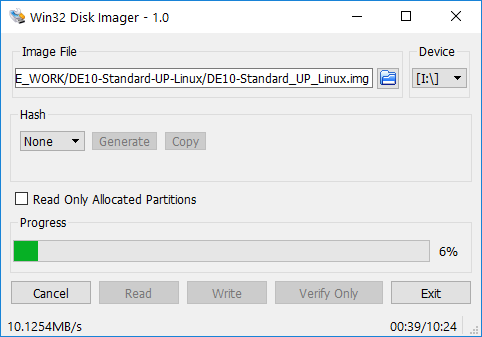
\includegraphics[scale = 0.7]{figures/Win32DiskImager1.png}
\end{center}
\caption{The Win32 Disk Imager program.}
\label{fig:win32_disk_imager}
\end{figure}
\item Select the drive letter corresponding to the SD-card under \texttt{Device}, 
as indicated in Figure~\ref{fig:win32_disk_imager}.
\item Select the \textit{DE1-SoC-UP-Linux.img} image under \texttt{Image File}, as shown in 
Figure~\ref{fig:win32_disk_imager}. This image file can be found following the
instructions in Section~\ref{sec:image}.
\item Click \texttt{Write} to write the microSD card. If prompted to confirm the overwrite, 
press \texttt{yes}. Once the writing is complete, you will see the success dialog shown in 
Figure~\ref{fig:win32_disk_imager_4}.
\begin{figure} [h]
\begin{center}
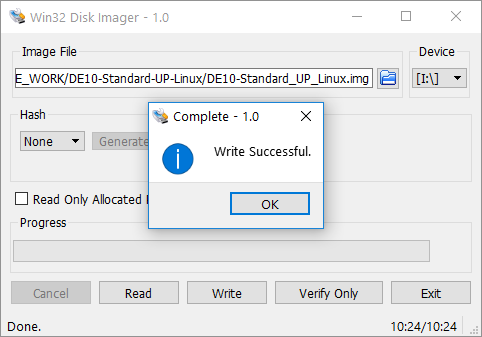
\includegraphics[scale = 0.7]{figures/Win32DiskImager4.png}
\end{center}
\caption{Writing a file to the microSD card using Win32 Disk Imager.}
\label{fig:win32_disk_imager_4}
\end{figure}

\end{enumerate}

\subsubsection{Preparing a MicroSD Card Using macOS or Linux}

Another popular program for writing disk images is {\it Etcher}, which can be freely
downloaded and installed from \texttt{https://www.balena.io/etcher}. This program is 
available for both macOS and Linux (and also for MS Windows). Some instructions for using 
this tool are provided below:

\begin{enumerate}

\item Insert a microSD card (8 GB or larger) into your computer's SD-card reader/writer,
and then launch the etcher (also called {\it balenaEtcher}) program, as illustrated in
Figure~\ref{fig:etcher}.

\begin{figure} [b]
\begin{center}
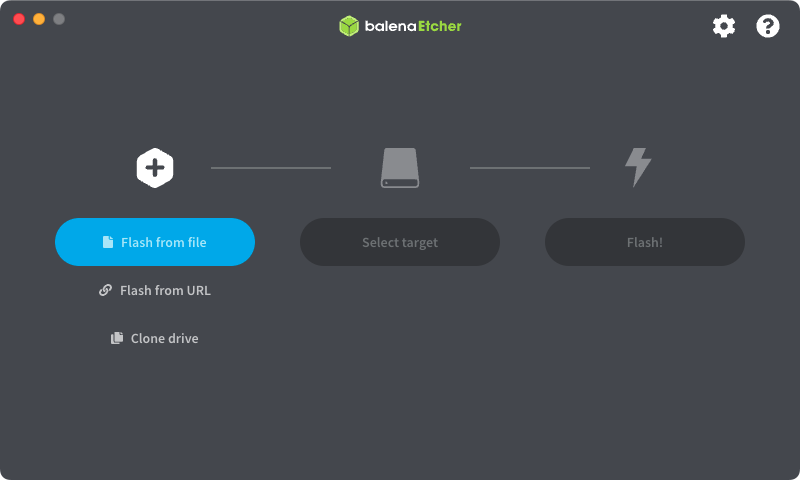
\includegraphics[scale = 0.45]{figures/etcher.png}
\end{center}
\caption{The Etcher application program.}
\label{fig:etcher}
\end{figure}
\item Click on \texttt{Flash from file} and browse to select the 
\textit{DE1-SoC-UP-Linux.img} image file.  This image file can be found following the
instructions in Section~\ref{sec:image}.
\item Click on \texttt{Select target} to choose your flash drive.
\item Click on \texttt{Flash!}. Once the writing is complete, you can remove the disk from
the host computer.

\end{enumerate}

\subsection{Setting up your DE1-SoC Board for use with Linux}

First ensure that your DE1-SoC board is powered off, and then insert the Linux 
microSD card into the microSD card slot. Before turning on the board, ensure that the
\texttt{Mode Select} (MSEL) switches found on the underside of the board match the settings shown 
in Figure~\ref{fig:msel}. These settings configure the Cyclone V SoC chip so as to allow the 
ARM processor to program the FPGA. It is necessary to have these settings because the Linux 
image programs the FPGA as part of its boot-up process. We should note that making this
change to the MSEL switches does not prevent the FPGA from being programmed using other
methods, such as via the Intel Quartus Prime Programming tool.

\begin{figure} [H]
\begin{center}
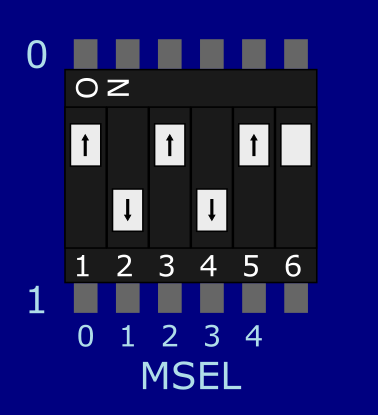
\includegraphics[scale = 1.00]{figures/MSEL.png}
\end{center}
\caption{Configuring the MSEL switches of your DE1-SoC board.}
\label{fig:msel}
\end{figure}

\section{Connecting your DE1-SoC Board to a Host Computer}

Before booting Linux, you should first connect your DE1-SoC board to a host computer.
There are two main methods of communicating between the DE1-SoC board and the host
computer: using a {\it USB-to-UART} serial connection, and using a {\it network} connection.
We will first discuss the serial connection, because when Linux boots it prints status
messages to the {\it serial console terminal}. Network connections are discussed in 
Section~\ref{sec:conn_network}.

\subsection{Connecting to the Host Computer using a USB-to-UART Connection}
\label{sec:conn_USB}

The Linux image has been configured to send and receive text to/from a host computer via a 
USB-to-UART cable. The USB cable is connected to a {\it UART-to-USB} port, which can be used to 
send and receive text messages. Via the host computer, we can access a \textit{serial terminal
console} to display this text. Various programs are available for connecting to serial
ports, depending on your host computer operating system.

\subsubsection{Connecting to a Serial Port using a Microsoft* Windows* Host Computer}

Under MS Windows a popular program for accessing serial ports is {\it putty}, which is
free to download and install from the Internet. 
In the following discussion we assume that you have installed {\it putty} on your host computer.
If you use a different terminal program, then the instructions below
would need to be modified accordingly. Connect the UART-to-USB port of your DE1-SoC board 
to your host computer; you can use the mini-USB cable that is normally supplied with the 
board, or an equivalent cable. To identify the
correct port, look for a small label on the board that reads \texttt{UART}. It can be found 
in the area of the board near the \texttt{RJ45} Ethernet port. If this is your first 
time connecting to the UART-to-USB port, then you may have to install its device driver 
on your host computer. If your host computer's operating system does not automatically 
install the driver, then you can search for it on the Internet. An appropriate search 
string is {\sf FT232R UART USB 
Driver}, which should locate the driver on a website called {\it ftdichip.com}.

On a Windows host computer, serial communication ports such as the UART-to-USB 
are treated as \texttt{COM} ports. Since a host computer may have multiple COM ports, 
each one is assigned a unique identifying number. The number assigned can be 
determined by viewing the list of COM ports in the Windows
\textit{Device Manager}. Figure \ref{fig:putty_0} shows the \textit{Device Manager's} list of 
available COM ports on one particular computer. Here, there is only one COM port (the UART-to-USB)
which is assigned the number 3 (COM3). If more COM ports were listed, then the UART-to-USB
port could be determined by disconnecting and reconnecting the cable to see which COM port 
disappears, then reappears, in the list.

\begin{figure}[H]
   \begin{center}
       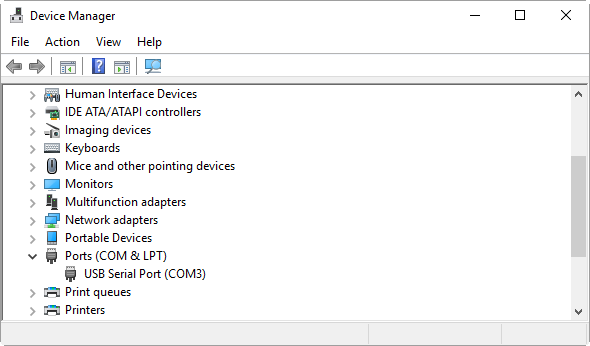
\includegraphics[scale=0.7]{figures/fig_putty_tut_0}
   \end{center}
   \caption{Determining the COM port of the UART-to-USB connection in Device Manager.}
	\label{fig:putty_0}
\end{figure}

\subsubsection{Using Putty}

Start the Putty program. Now that the serial device (COM port) corresponding to the 
UART-to-USB connection is known, Putty can be configured to connect to it. 
Figure \ref{fig:putty_1} shows the
main window of Putty. In this window, the {\it Connection type} has been set to
\texttt{Serial}, and 
COM3 has been specified in the \texttt{Serial line} field. 

\begin{figure}[H]
   \begin{center}
       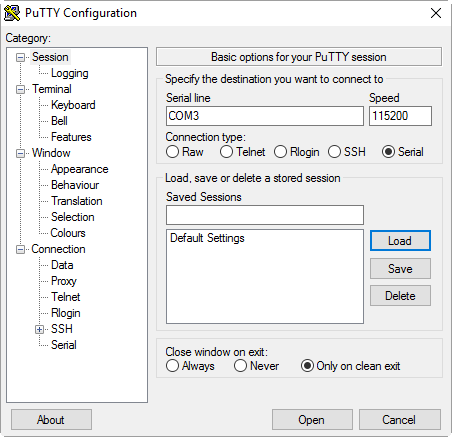
\includegraphics[scale=0.7]{figures/fig_putty_tut_1}
   \end{center}
   \caption{Putty's main window.}
	\label{fig:putty_1}
\end{figure}

Some additional details about the UART-to-USB connection must be entered by selecting the 
\texttt{Serial} panel in the \texttt{Category} box on the left side of the window. The
\texttt{Serial}
panel is shown in Figure \ref{fig:putty_2}. These settings must match the configuration of the 
UART. As shown in the figure set the speed (baud rate) to 115200 bits per second, data
bits to 8, stop bits to 1, and parity and flow control to \textit{none}. 

Once all of the serial-line settings have been entered, press \texttt{Open} to start the
{\it Terminal}. Now, turn on the power to your DE1-SoC board. You should now see a stream 
of text in the Putty terminal that shows the status of the Linux boot process, as displayed in 
Figures~\ref{fig:putty_3} and~\ref{fig:putty_4}. Once Linux has finished booting, you will be 
logged in to the Linux serial console terminal as the \textit{root} user. Being logged 
in as root means that you that have administrator-level privileges, which allow you to modify 
settings and execute privileged programs.

In the {\it Terminal} window press \texttt{Enter} on your keyboard to see that the
terminal responds.  Type a Linux command such as \texttt{ls}, which shows a listing of 
directories and files. 

~\\
\begin{figure}[H]
   \begin{center}
       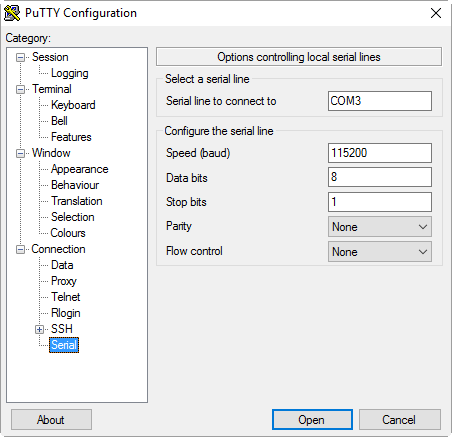
\includegraphics[scale=0.8]{figures/fig_putty_tut_2}
   \end{center}
   \caption{Putty's configuration window for serial communication settings.}
	\label{fig:putty_2}
\end{figure}

\begin{figure}[H]
   \begin{center}
       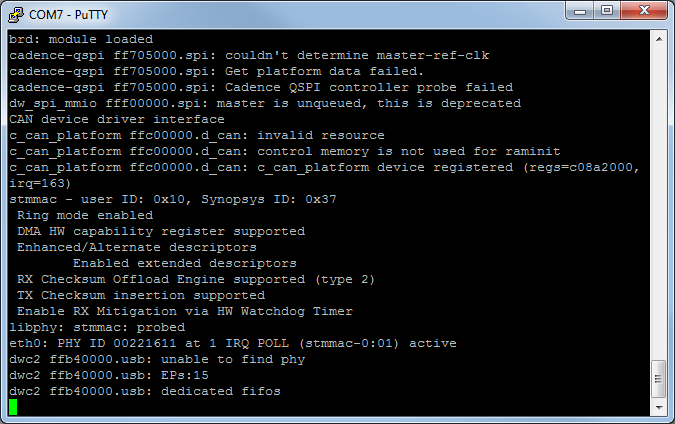
\includegraphics[scale=0.7]{figures/fig_putty_tut_3}
   \end{center}
   \caption{Putty terminal displaying text output as the Linux kernel boots.}
	\label{fig:putty_3}
\end{figure}

\begin{figure}[H]
   \begin{center}
       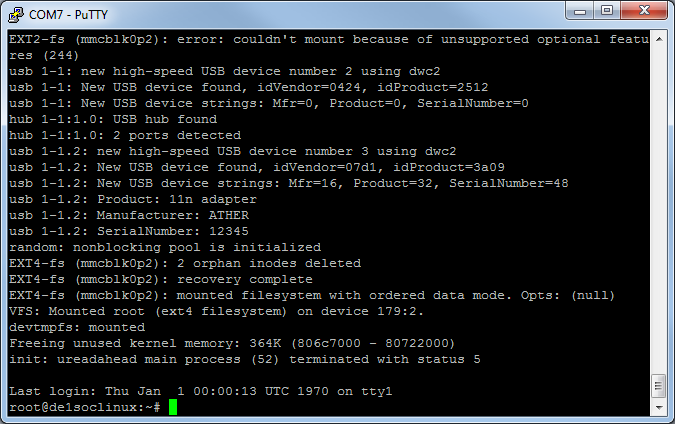
\includegraphics[scale=0.7]{figures/fig_putty_tut_4}
   \end{center}
   \caption{The Linux command line prompt showing the root ('\#') logon.}
	\label{fig:putty_4}
\end{figure}

\subsubsection{Using a Linux* Host Computer}

You should read this section if your host computer is running a version of Linux.
On a Linux host computer, serial communication devices such as the UART-to-USB are treated 
as \textit{teletype} (tty) devices. Since there can be multiple tty devices connected to
the host computer, each tty device is assigned a unique identifier. The name assigned to your 
UART-to-USB connection
can be determined by running the command \texttt{dmesg | grep tty} as shown in 
Figure~\ref{fig:dmesg}. In the figure, you can see that the UART-to-USB chip (the manufacturer's
name for this device is \textit{FTDI USB Serial Device converter}) has been assigned the name 
ttyUSB0.

\begin{figure}[H]
   \begin{center}
       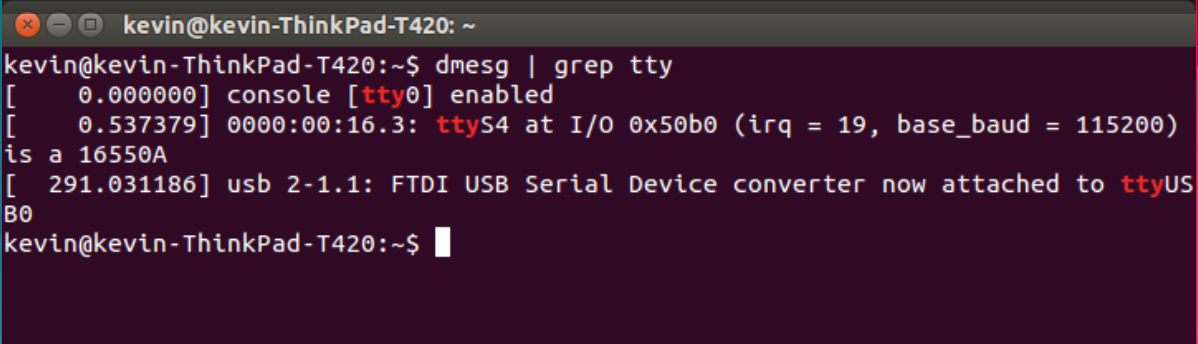
\includegraphics[scale=0.5]{figures/new_tty.png}
   \end{center}
   \caption{Determining the tty device that corresponds to the UART-to-USB connection.}
	\label{fig:dmesg}
\end{figure}

Once you have determined which tty port is connected to your DE1-SoC board, you can run a
serial communications program to connect to the Linux serial console terminal on the
board. If you use the putty program, which is available for Linux, then you can follow
similar instructions given above for MS Windows computers. But if you choose a different
serial communications program (several alternative programs are available), then you will
need to adapt your procedures accordingly.

\subsubsection{Using a macOS Host Computer}

You should read this section if your host computer is running a version of macOS.
On a macOS host computer, serial communication devices such as the UART-to-USB are treated 
as \textit{teletype} (tty) devices. Since there can be multiple tty devices connected to
your computer,  each one is assigned a unique identifier.
To determine which tty port corresponds to your USB-to-UART port, open the macOS 
{\it Terminal} application and then type the command \texttt{ls /dev/tty.*}. An example of
the output produced by this command is shown in Figure~\ref{fig:macOSTerminal}. It shows
a USB-to-UART tty device called \texttt{/dev/tty.usbserial-AL04C11T.}

\begin{figure}[H]
   \begin{center}
       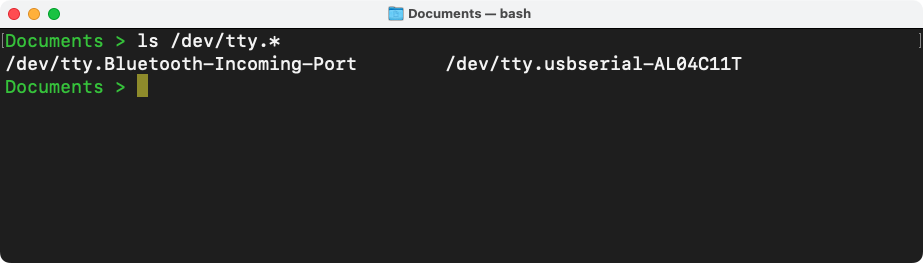
\includegraphics[scale=0.5]{figures/macOSTerminal.png}
   \end{center}
   \caption{Determining the tty device under macOS.}
	\label{fig:macOSTerminal}
\end{figure}

A number of application programs are available under macOS to connect to tty ports. Here
we will use the built-in application called {\it screen}. To connect to the identified
serial port, we need to specify its identifier and baud rate, which can be done by
executing in a macOS Terminal the command

\texttt{screen /dev/tty.usbserial-AL04C11T 115200}

This command makes a connection to the Linux serial console terminal on the DE1-SoC board. 
If you turn on the DE1-SoC board after running this \texttt{screen} command, then you will
see the status messages that are printed to the serial console while Linux boots. After
the boot process is finished, press the \texttt{return} keyboard key to see the Linux
prompt from the DE1-SoC board, and then execute a command such as \texttt{ls} to see 
the files and directories that are available.

You can execute the command \texttt{man screen} to learn how to control the
\texttt{screen} application. To execute a \texttt{screen} command you have to first type
the {\it escape} sequence \texttt{control-A} (abbreviated here as \texttt{C-A}), 
followed by the command. For example, to see a list of all \texttt{screen} commands you can 
type \texttt{C-A ?}. To quit a \texttt{screen} session that is connected to Linux on the
DE1-SoC board you can type \texttt{C-A k}, and then type \texttt{y} in answer to the
prompt from \texttt{screen} ``\texttt{Really kill this window [y/n]}''.

\subsection{Connecting to the Host Computer using a Network}
\label{sec:conn_network}

As discussed in the previous section, it is useful to establish a USB-to-UART connection 
to the DE1-SoC board, because this connection provides access to the Linux serial console 
terminal.  However, this serial connection offers limited functionality, because of its 
relatively slow speed of operation. In this section we show how to establish a high-bandwidth 
communication link between your host computer and the DE1-SoC board, by using a 
{\it network connection}. The network connection allows useful capabilities, such as 
{\it secure shell} (ssh), {\it virtual network computing} (VNC), and {\it file transfer
protocol} (FTP) to used with Linux on the DE1-SoC board. There are two ways to establish 
the network connection: using an Ethernet cable, and using a WiFi adapter. 
Both methods are discussed below.

\subsubsection{Connection using an Ethernet Cable}

Although many types of network setups can be created with Ethernet cables, for this discussion
we assume that your DE1-SoC board is directly plugged into an Ethernet port on your host
computer, via either a built-in Ethernet port or a USB-to-Ethernet adaptor. Use the
\texttt{RJ45} port on the DE1-SoC board to make the Ethernet connection. If you
have some other type of Ethernet setup, then the instructions provided here might
have to be modified somewhat. If there is no Ethernet port available on your host computer, 
then you have to connect to the board by using a USB-to-UART serial connection, as discussed
in Section \ref{sec:conn_USB}. It is recommended to use an Ethernet connection, as 
functionality is limited when using only a serial connection to the board. 

The DE1-SoC board is set up to use either of two {\it IPv4} network addresses via 
Ethernet: \texttt{192.168.0.123} and \texttt{192.168.1.123}. For an Ethernet port on 
the host computer to connect to the DE1-SoC board, this Ethernet port's network address 
must be on the same {\it subnet}. This means that the Ethernet port's network address must 
be of the form \texttt{192.168.0.}{\it xxx} or \texttt{192.168.1.}{\it xxx}. 
The steps required to complete the Ethernet connection are described below.

You first need to determine the {\it IPv4} address of the Ethernet port that is connected to your
DE1-SoC board. The procedures for making network settings for Ethernet
ports varies for different host computer operating systems, but these procedure can 
be easily found by searching for them on the Internet. Using these procedures, open the 
network settings user interface on your host computer. 

If your host computer has more than one Ethernet port, then you will see multiple ports in
your network settings user interface. To determine which port is plugged into the DE1-SoC board,
a workable approach is to unplug/re-plug the cable that is connected to the board,
and observe which Ethernet port is
affected. Once your have identified the correct Ethernet port, examine its {\it IPv4} address.
If the address is on subnet \texttt{192.168.0} or \texttt{192.168.1}, then you do not need
to modify the address of the port and can skip to Section~\ref{sec:connecting}. 
Otherwise, you need to change the {\it IPv4} address of your Ethernet port, as discussed
below. 

Configure the Ethernet port that you are using to connect to your DE1-SoC board to 
have a {\it manually-set IPv4} address (the default setting is usually to have an address 
set automatically by using a {\it Dynamic Name Server} (DNS)). Set the \texttt{IPv4} address 
to \texttt{192.168.0.xxx}, and set the \texttt{Subnet} mask to \texttt{255.255.255.0}. 
For \texttt{xxx} use any address that is not already assigned to a device on your network
(for example, use \texttt{xxx} = 111 if this address is not already in use). If a
\texttt{Default gateway} is shown in the settings, leave this field blank.

Once you have established the correct {\it IPv4} address, you can connect to the DE1-SoC
board as described in Section~\ref{sec:connecting}. In some situations it is possible that
you might not have an available Ethernet port whose address can be set as needed.
In such an instance, an alternative approach is to modify the 
{\it IPv4} address of the DE1-SoC board, using the procedure discussed below.

\subsubsection*{Changing the IP address of a DE1-SoC Board}

To change the IP address of your DE1-SoC board you have to first connect your host computer
to the board via a USB cable, as described in Section~\ref{sec:conn_USB}. Then, using the 
Linux serial console terminal on the DE1-SoC board execute the \texttt{ifconfig} 
command. The \texttt{ifconfig} command shows you the current IP address(es) that are
assigned to the board. You can use \texttt{ifconfig} to change the IP address. For example, 
let's assume that your host computer's IP address is \texttt{192.168.86.33}. Then, you could 
use the command \texttt{ifconfig eth0 192.168.86.123} to change your board's IP address.
In this command \texttt{123} is just an example---it can be any number that is not
already being used in your router's subnet. Note that \texttt{eth0} is the name of an ethernet
port that is available to Linux.

\subsubsection{Connecting to the Host Computer using a WiFi Adapter}
\label{sec:WiFi}
If you wish to make a network connection to your DE1-SoC board using a WiFi adapter, then 
you first have to connect your host computer to the board via a USB cable
as discussed in Section~\ref{sec:conn_USB}. Then, you can use the Linux serial console
terminal to make the needed settings. The discussion below assumes that you have 
successfully opened the required console window. 

Linux supports a variety of USB WiFi adapters. At the time of writing this
tutorial WiFi adapters supported by Linux kernel version 3.18 have been tested. Other WiFi
adapters may also be usable, but drivers may need to be manually installed.

Plug your WiFi adapter into a USB port on your DE1-SoC board. To join a desired WiFi network, 
you can run the following script in the Linux Terminal 
window: \texttt{connect\_wpa <ssid> <password>.} This script can 
be found in the directory {\it /home/root/misc} in the Linux filesystem. Your DE1-SoC 
board should become connected to your WiFi network after a few moments.

Instead of using the \texttt{connect\_wpa} script, it is possible to run the Linux commands
included in the script manually. First, using the Terminal window connected to Linux on
your DE1-SoC board, create an ASCII text file in a directory of your choosing. Give the file 
a name ending in .{\it conf}, such as {\it mywifi.conf}. This file has to contain the lines

\begin{lstlisting}
network={
	ssid="<ssid>"
	psk="<password>"
}
\end{lstlisting}

The first character on each of the second and third lines is a {\it tab} character.
Now, run the following Linux commands:

\begin{lstlisting}
stop network-manager
wpa_supplicant -B -iwlan0 -c./mywifi.conf -Dnl80211
dhclient wlan0
\end{lstlisting}

The wireless interface on your DE1-SoC board might not be {\it wlan0}. To
determine the correct name, use the Linux command \texttt{iwconfig}. You can check the IP address 
assigned by the WiFi router using the Linux \texttt{ifconfig} command. Then, you can then use 
this IP address, as described in Section~\ref{sec:VNC}, to connect to the VNC server from a 
host computer on the same WiFi network.

\subsection{Using the Network Connection}
\label{sec:connecting}

This section assumes that you have set up a working Ethernet or WiFi network connection 
between your host computer and Linux on the DE1-SoC board.  As a first step to verify that
the network connection is established, execute the \texttt{ping} command on your host
computer, as illustrated by the example in Figure~\ref{fig:ping}. If no data bytes are 
returned to the host computer from the DE1-SoC board, then you should revisit the procedures
described above to make a working network connection.

\begin{figure}[H]
   \begin{center}
       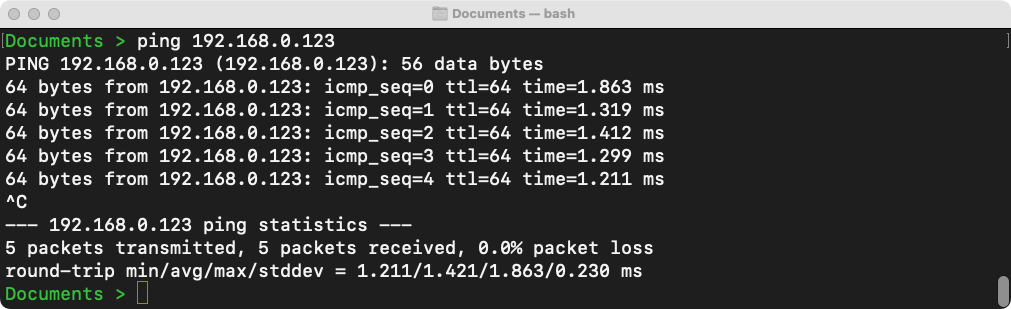
\includegraphics[scale=0.4]{figures/ping.png}
   \end{center}
   \caption{Using the \texttt{ping} command.}
	\label{fig:ping}
\end{figure}

\subsubsection{Using Secure Shell (ssh)}
\label{sec:ssh}

The {\it secure shell} (ssh) application allows you to login to Linux on the DE1-SoC
board via your network connection.  An example of an \texttt{ssh} command is

\texttt{ssh -l root 192.168.0.123}

Upon executing this command, Linux on the DE1-SoC board should prompt for the \texttt{root} 
login password. Type \texttt{password} in response and then press the \texttt{return} key. 
Once logged in to the DE1-SoC board you can execute any Linux command via its command line 
interface (CLI).  When finished, you can log out by typing \texttt{exit}.

\subsubsection{Using the VNC Server}
\label{sec:VNC}
The DE1-SoC-UP Linux image has been configured to include 
a graphical user interface (GUI) via a virtual network computing (VNC) server. The 
VNC server transmits a copy of the GUI to a network port, which allows the host computer 
to use the GUI via a network connection. The network port used 
by the VNC server is \texttt{5901}, and the password for the VNC server is set to
\texttt{password}.

A variety of client programs are available for communicating with a VNC server, depending
on your host computer operating system, as discussed below.

\subsubsection{Using VNC on MS Windows}

One popular VNC program for use with MS Windows is the {\it RealVNC* Viewer}, which is 
free to use. Installing and running this program opens the dialog shown in Figure~\ref{fig:VNC_1}.
The VNC Server address is specified assuming that the default DE1-SoC {\it IPv4} address
\texttt{192.168.0.123} is being used, and port \texttt{5901} is specified as required. Clicking 
on the {\it Connect} button opens another dialog that prompts for the 
password. Providing the password (which is just set to \texttt{password} in our case) opens the 
VNC window shown in Figure~\ref{fig:VNC_2}. In the figure we have opened the {\it Terminal}
command prompt window inside the VNC Viewer and typed the Linux command \texttt{pwd}.

The VNC Server supports four different screen sizes. Using a {\it Terminal} command prompt 
window in the VNC Viewer the screen size can be changed with the \texttt{xrandr} command. 
You can type \texttt{xrandr~-s~0} to select the smallest screen size, and \texttt{xrandr -s 3}
to choose the largest size.

The Linux image includes many application programs that can be accessed via using VNC.
It provides several text editors, including {\it gedit}, {\it Emacs}, {\it vim}, and 
{\it gvim}.  It also includes the {\it Code::Blocks} integrated development environment. 
This tool provides a source-level debugger that can be used to develop applications programs. In
Appendix A we provide a short tutorial that shows how to use {\it Code::Blocks} to develop
C programs that run on the ARM processor under Linux. 

~\\
\begin{figure}[H]
   \begin{center}
       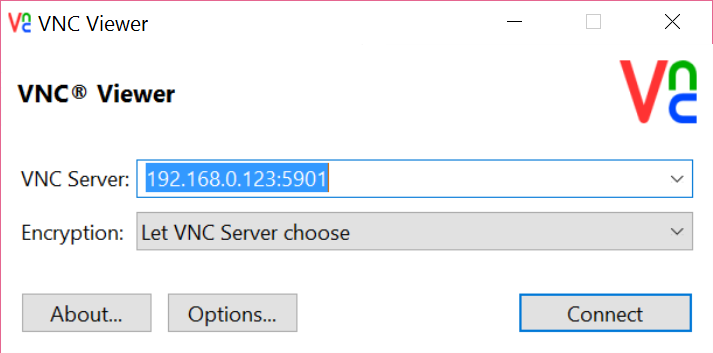
\includegraphics[scale=0.5]{figures/VNC_1}
   \end{center}
   \caption{The RealVNC opening dialog.}
	\label{fig:VNC_1}
\end{figure}

\begin{figure}[H]
   \begin{center}
       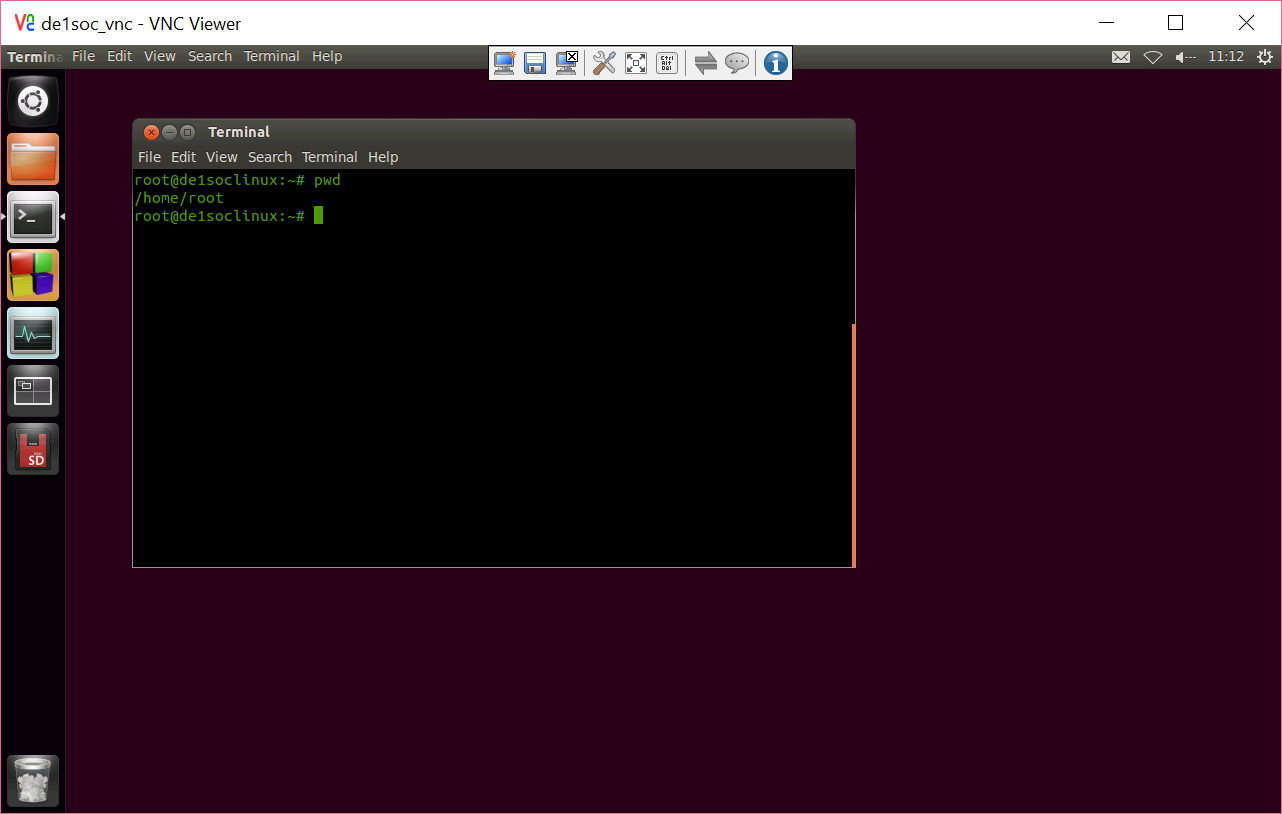
\includegraphics[scale=0.5]{figures/VNC_2}
   \end{center}
   \caption{The main RealVNC window.}
	\label{fig:VNC_2}
\end{figure}

\subsubsection{Using VNC on Linux}

The {\it Remmina} application is a popular VNC viewer for Linux host computers.
Figure~\ref{fig:Remmina} gives an example of a Remmina GUI window. In the figure we have 
selected the \texttt{VNC} protocol and specified the address and port number 
(\texttt{192.168.0.123:5901}) needed for the DE1-SoC board. These settings
open the VNC server window as discussed above for Figure~\ref{fig:VNC_2}.
Remmina can be freely downloaded from the Internet and is included by default in many
Linux distributions.

~\\
\begin{figure}[H]
   \begin{center}
       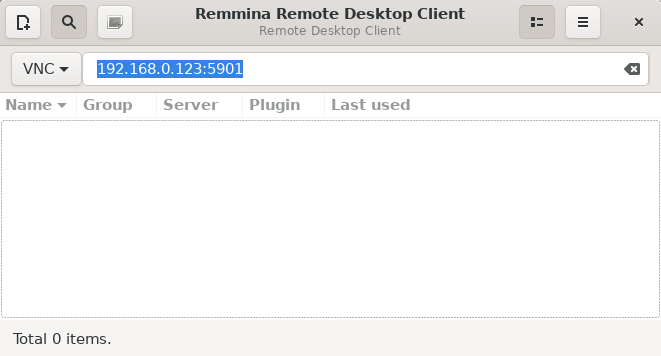
\includegraphics[scale=.8]{figures/remmina.png}
   \end{center}
   \caption{The Remmina window.}
	\label{fig:Remmina}
\end{figure}

\subsubsection{Using VNC on macOS}

For macOS there is a built-in VNC viewer. Executing the command

\texttt{open vnc://192.168.0.123:5901}

causes Linux on the DE1-SoC board to prompt for the VNC password. Responding with
\texttt{password} establishes a VNC logon and opens the VNC server window 
illustrated in Figure~\ref{fig:VNC_2}.

\subsubsection{Transferring Files to/from the Host Computer}
\label{sec:ftp}

Files can be transferred between the host computer and Linux on the DE1-SoC board over the
network connection. One simple method of copying files is to use the {\it secure copy} (scp)
program. Instructions for using scp can be obtained from the Internet or, on macOS and
Linux, by executing \texttt{man scp}. Another method of copying files is to use the 
{\it file transfer protocol} (FTP), described below.  

The Linux image includes an {\it FTP} Server that can be used to transfer files
between the host computer and the DE1-SoC board. The FTP server uses the secure FTP
(SFTP) protocol and uses {\it Port 22} for the network connection. The login 
{\it Username} for the FTP Server is {\it root}, and the password is {\it password}. An
easy-to-use FTP client for Windows, macOS, and Linux host computers is {\it FileZilla}, 
available from {\it https://filezilla-project.org/}.

\subsubsection{Accessing the Internet}
\label{sec:internet}

It is possible to access external IP addresses on the Internet from your DE1-SoC board. 
To do so, connect your DE1-SoC board using an Ethernet cable directly (or through an
Ethernet switch) to your Internet router. Open a serial port connection to your DE1-SoC
board, as described in Section~\ref{sec:conn_USB}, and execute the commands

\begin{verbatim}
ifconfig eth0 0.0.0.0 0.0.0.0
dhclient eth0
\end{verbatim}

These commands set up the {\it eth0} port as a DHCP client of the router. The {\it eth0} port 
will obtain an automatically-assigned IP address that allows Internet access.

\section{Developing Linux* Programs for your DE1-SoC Board}
\label{sec:linux_programs}

In this section you will learn how to develop programs that can run under Linux on 
your DE1-SoC board. There are two options for developing a Linux program in a language such
as C for your DE1-SoC board. The first is to compile the C code by using the \texttt{gcc}
compiler that is provided with the Linux running on the board. This approach is called 
\textit{native compilation}. This is the method that we use in this tutorial. The second option is 
to compile your program on a host computer, and then transfer the resulting executable onto 
the Linux filesystem (microSD card). This approach, which is called \textit{cross compilation}, 
is not used in this tutorial.

To perform native compilation you need to compile your C code by using the \texttt{gcc} compiler 
provided with Linux that is running on the board. However, this process does not require you to
actually {\it type} the C code with a text editor running under Linux. Instead, you could type
your C source code on a host computer, such as a Windows PC, and then transfer the file
onto your Linux filesystem (microSD card) to compile it. This approach is illustrated in 
Figure~\ref{fig:dev_setup}. It shows a text editor running on the host computer, which is being
used to type the contents of a C source-code file. In this case the {\it gvim} editor is
being used, but you could run whatever text editor you prefer on the host computer. 
Figure~\ref{fig:dev_setup} also depicts an {\it ftp} program being used to transfer the
source-code file to Linux. In this ftp program, files on the host computer are listed in the 
left-hand side of the window, and files on the Linux filesystem (microSD card) are listed on
the right-hand side. In the figure we are running the {\it Filezilla*} program, but any 
ftp client on the host computer can be used. Finally, the figure depicts a {\it Terminal} 
window connected to Linux. The Terminal provides access to the Linux 
{\it command line interface} (CLI). The CLI allows you to execute Linux programs, such 
as the C-compiler, on the DE1-SoC board. The Terminal window in this case is provided 
by {\it putty}. It communicates with the DE1-SoC board via a USB cable, discussed in 
Section~\ref{sec:conn_USB}. You might instead use an {\it ssh} connection to the DE1-SoC board
via a terminal on your host computer. An {\it ssh} connection gives a much higher bandwidth in
comparison to {\it putty}, because {\it ssh} (as well as {\it ftp}) communicates with the board
via a network connection, discussed in Section~\ref{sec:conn_network}

An alternative to the setup in Figure~\ref{fig:dev_setup} is to use the VNC Viewer as
depicted in Figure~\ref{fig:VNC_2}. In this case you would not need to use the Terminal
window that is connected via USB, because an equivalent Terminal window can be opened directly
in the VNC Viewer window. You could choose to run one of the editors provided with the
Linux image within the VNC Viewer, to create source-code files directly on the Linux 
filesystem (microSD card). Or, you could still create files on the host computer and then
transfer them to Linux via ftp.

\subsection{Native Compilation on the DE1-SoC Board}
\label{sec:native_compile}

As mentioned previously, when a program is compiled on a system to run on the same architecture
as that of the system itself, the process is called {\it native compilation}. In this section,
we will be natively compiling a program through the Linux command-line interface, using its 
built-in compilation tool-chain.

\begin{figure}[H]
   \begin{center}
       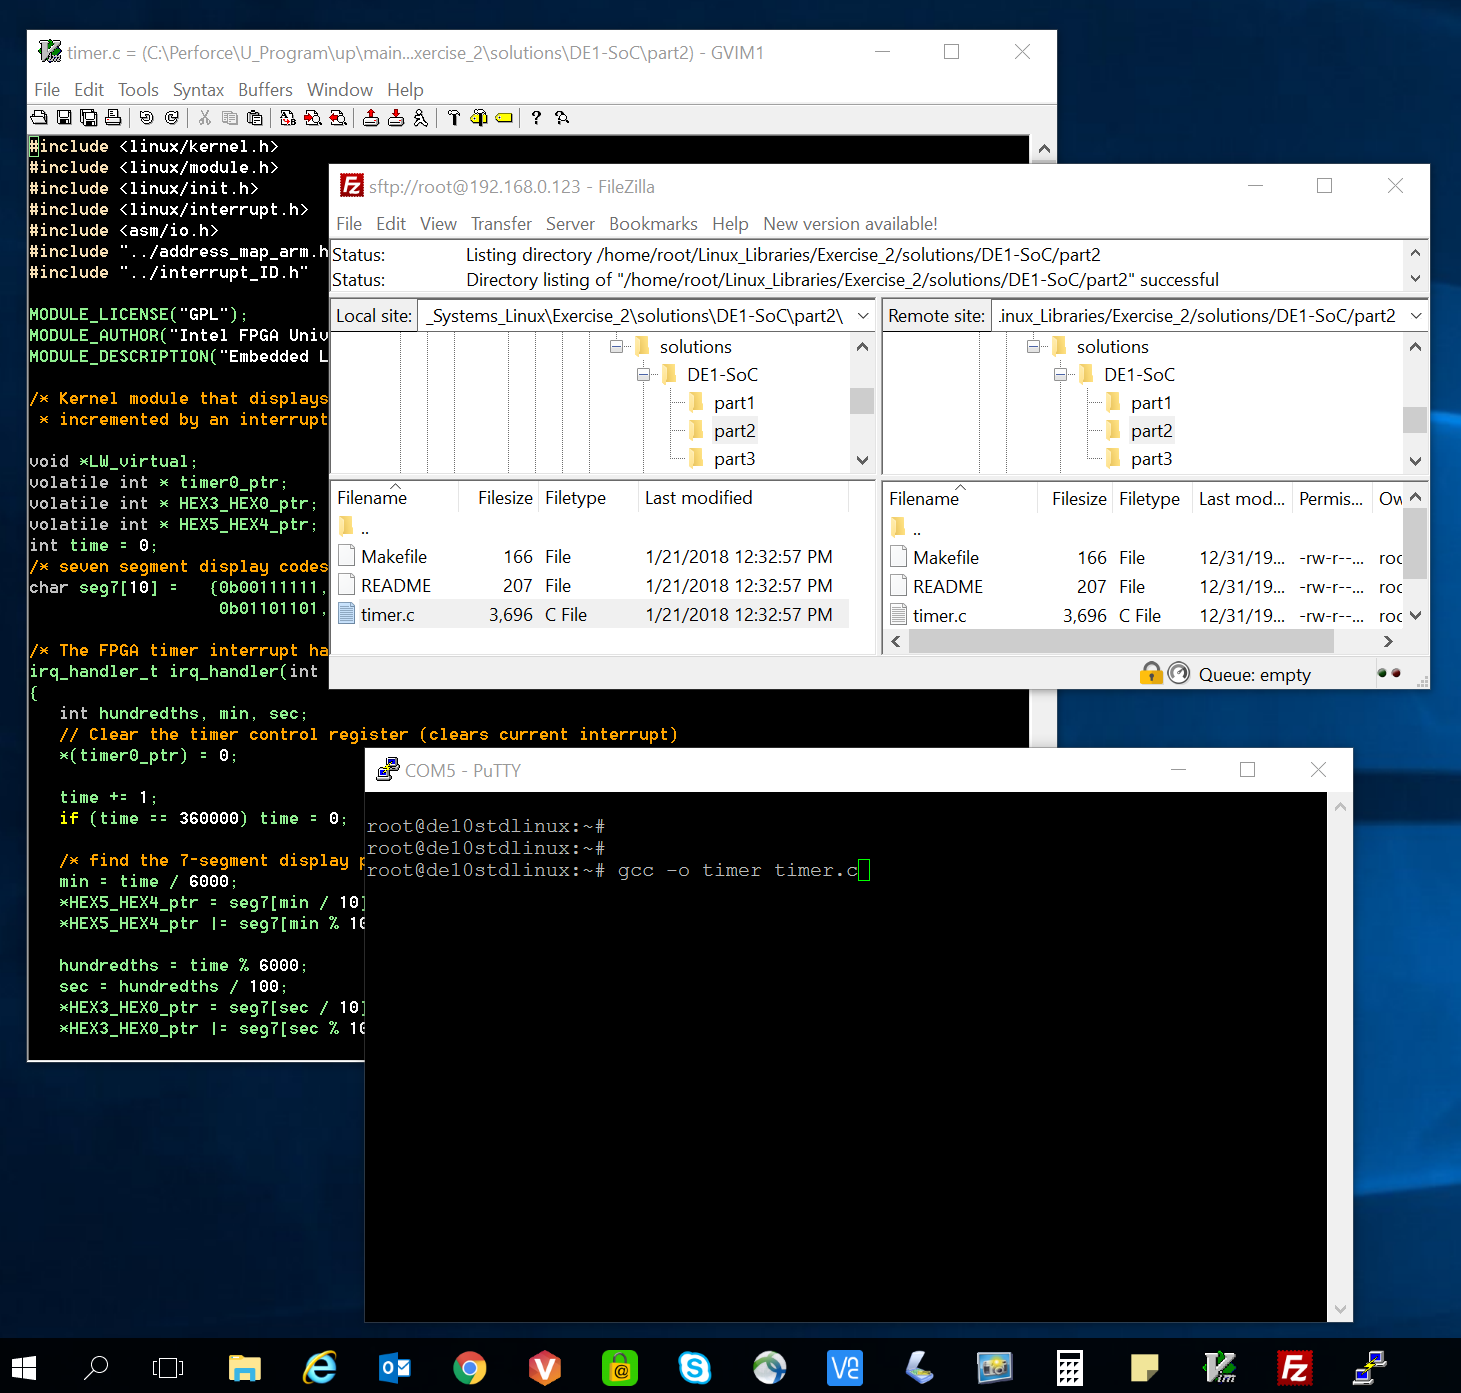
\includegraphics[width=\textwidth]{figures/dev_setup_2.png}
   \end{center}
   \caption{Using a host computer to write code, and ftp to transfer to Linux.}
	\label{fig:dev_setup}
\end{figure}

To demonstrate native compilation, we will compile a simple "hello world" program. The code 
for this program is shown in Figure~\ref{fig:helloworld_code}. You can also find the code 
in \textit{/home/root/tutorial\_files/helloworld/helloworld.c} of the Linux filesystem.

\lstset{language=C,numbers=left}
\begin{figure}[H]
\begin{center}
\begin{minipage}[t]{16 cm}
\begin{lstlisting}
#include <stdio.h>

int main(void){
   printf("Hello World!\n");
   return 0;
}
\end{lstlisting}
\end{minipage}
\end{center}
\vspace{-0.33in}\caption{The helloworld program}
\label{fig:helloworld_code}
\end{figure}

You can compile code using the Linux command-line interface. If you are using a USB cable
to connect to the DE1-SoC board, as discussed in Section~\ref{sec:conn_USB}, then use the
{\it putty} tool to open a {\it Terminal} window. If you are using the VNC Viewer, as 
described in Section~\ref{sec:conn_network}, then open a {\it Terminal} window in the GUI. 
In your {\it Terminal} window change the working directory to 
\textit{/home/root/tutorial\_files/helloworld}. 
Compile the program using the command \texttt{gcc helloworld.c -o helloworld}, as 
shown in Figure~\ref{fig:helloworld_native}. The \texttt{gcc} command invokes 
the \textit{GNU C Compiler}, which is an open-source compiler that is widely used to compile 
Linux programs. In our \texttt{gcc} command, we supply two arguments. The first is the source-code 
file, \texttt{helloworld.c}. The second is \texttt{-o helloworld} which 
tells the compiler to output an executable file named \textit{helloworld}. Once the compilation 
is complete, we can run the program by typing \texttt{./helloworld}. The program outputs the 
message "Hello World!", and then exits, as shown in Figure~\ref{fig:helloworld_native}.
~\\
\begin{figure}[H]
   \begin{center}
       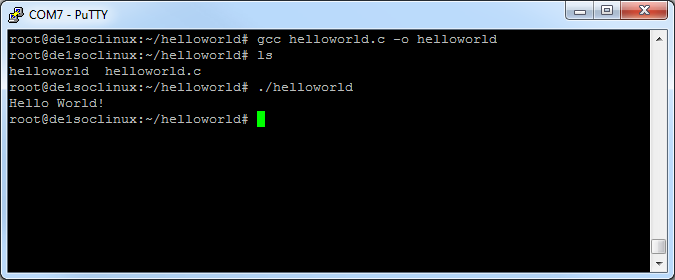
\includegraphics[scale=0.7]{figures/compilation_1}
   \end{center}
   \caption{Compiling and executing the \textit{helloworld} program through the command line.}
	\label{fig:helloworld_native}
\end{figure}

\subsection{Accessing Hardware Devices in the FPGA from a Linux* Program}

Programs running on the ARM processor in the {\it DE1-SoC-UP-Linux} OS can access hardware 
peripherals that are implemented in the FPGA. The ARM processor can access the FPGA
by using either the {\it HPS-to-FPGA} {\it bridge} or 
the {\it Lightweight HPS-to-FPGA} {\it bridge}. These bridges are mapped to regions 
in the ARM memory space. When an FPGA-side component (such as an IP core) is connected to one 
of these bridges, the component's memory-mapped registers are available for reading and writing 
by the ARM processor within the bridge's memory region. 

If we were developing a ``bare metal'' ARM program (a program that does not run on top of an 
operating system), then accessing peripherals in the FPGA that are mapped to a memory region
would be done by simply reading from, or writing to, the appropriate memory address. Examples 
of software programs that access memory-mapped peripherals in the FPGA can be found on the 
Intel FPGA University Program website in the document {\it Using the DE1-SoC Computer with ARM}. 
But when programs are being run under Linux it is not as straightforward to access 
memory-mapped I/O devices. This is because Linux uses a virtual-memory system, and therefore 
application programs do not have direct access to the processor's physical address space. 

To access physical memory addresses from a program running under Linux, you have to call the
Linux kernel function \texttt{mmap} and access the system memory device file \textit{/dev/mem}. 
The \texttt{mmap} function, which stands for {\it memory map},
maps a file into virtual memory. You could, as an example, use \texttt{mmap} to map a text file 
into memory and then access the characters in the text file by reading the virtual memory address 
span to which the file has been mapped. The system memory device file, \textit{/dev/mem}, is 
a special file that represents the physical memory of the computer system. An access into
this file at some offset is equivalent to accessing physical memory at the offset address. By 
using \texttt{mmap} to map the \textit{/dev/mem} file into virtual memory, we can map 
physical addresses to virtual addresses, allowing programs to access physical addresses. 
In the following section, we will examine a sample Linux program that uses \texttt{mmap} 
and \textit{/dev/mem} to access the Lightweight HPS-to-FPGA ({\it lwhps2fpga}) bridge's
memory span and communicate with an IP core in the FPGA.

\subsection{Example Program that uses an FPGA Hardware Device}
\label{sec:program_with_fpga_communication}

In this section, we describe an example of code in the C language that uses a hardware
device in the FPGA. The application program alters the state of the red LEDs on 
the DE1-SoC board. 
Recall that the \textit{DE1-SoC-UP} Linux distribution automatically downloads the
circuit that implements the \textit{DE1-SoC Computer} system into the FPGA 
during the boot process. The \textit{DE1-SoC Computer} 
includes a parallel port that is connected to the red LEDs on the board. This parallel port 
is attached to the \textit{lwhps2fpga} bridge, which is mapped in the ARM memory space starting 
at address \texttt{0xFF200000}. A number of I/O ports are mapped to the bridge's
address space, at different {\it offsets}, and the 
physical address of any port is given by \texttt{0xFF200000 + {\it offset}}. The offset
of the red LED port is 0, so its address is \texttt{0xFF200000 + 0x0 = 0xFF200000}.
The LED parallel port register interface consists of a single register, the \textit{data} 
register, which can be read to determine the current state of the LEDs, and written to 
alter the state. A diagram showing how the red LEDs are connected to the parallel port is shown 
in Figure~\ref{fig:LED}.

The code for the application program is given in Figure~\ref{fig:increment_leds_code}.
Each time this program is executed, the value displayed on the red LEDs
is incremented by one. The example code can be found on the Linux microSD card in the file
\textit{/home/root/tutorial\_files/increment\_leds/increment\_leds.c}. You can 
compile the code using a command such as \texttt{gcc -Wall increment\_leds.c -o
increment\_leds}, and then run the program with the command \texttt{./increment\_leds}.
The code is described below. 

\begin{figure}[H]
   \begin{center}
       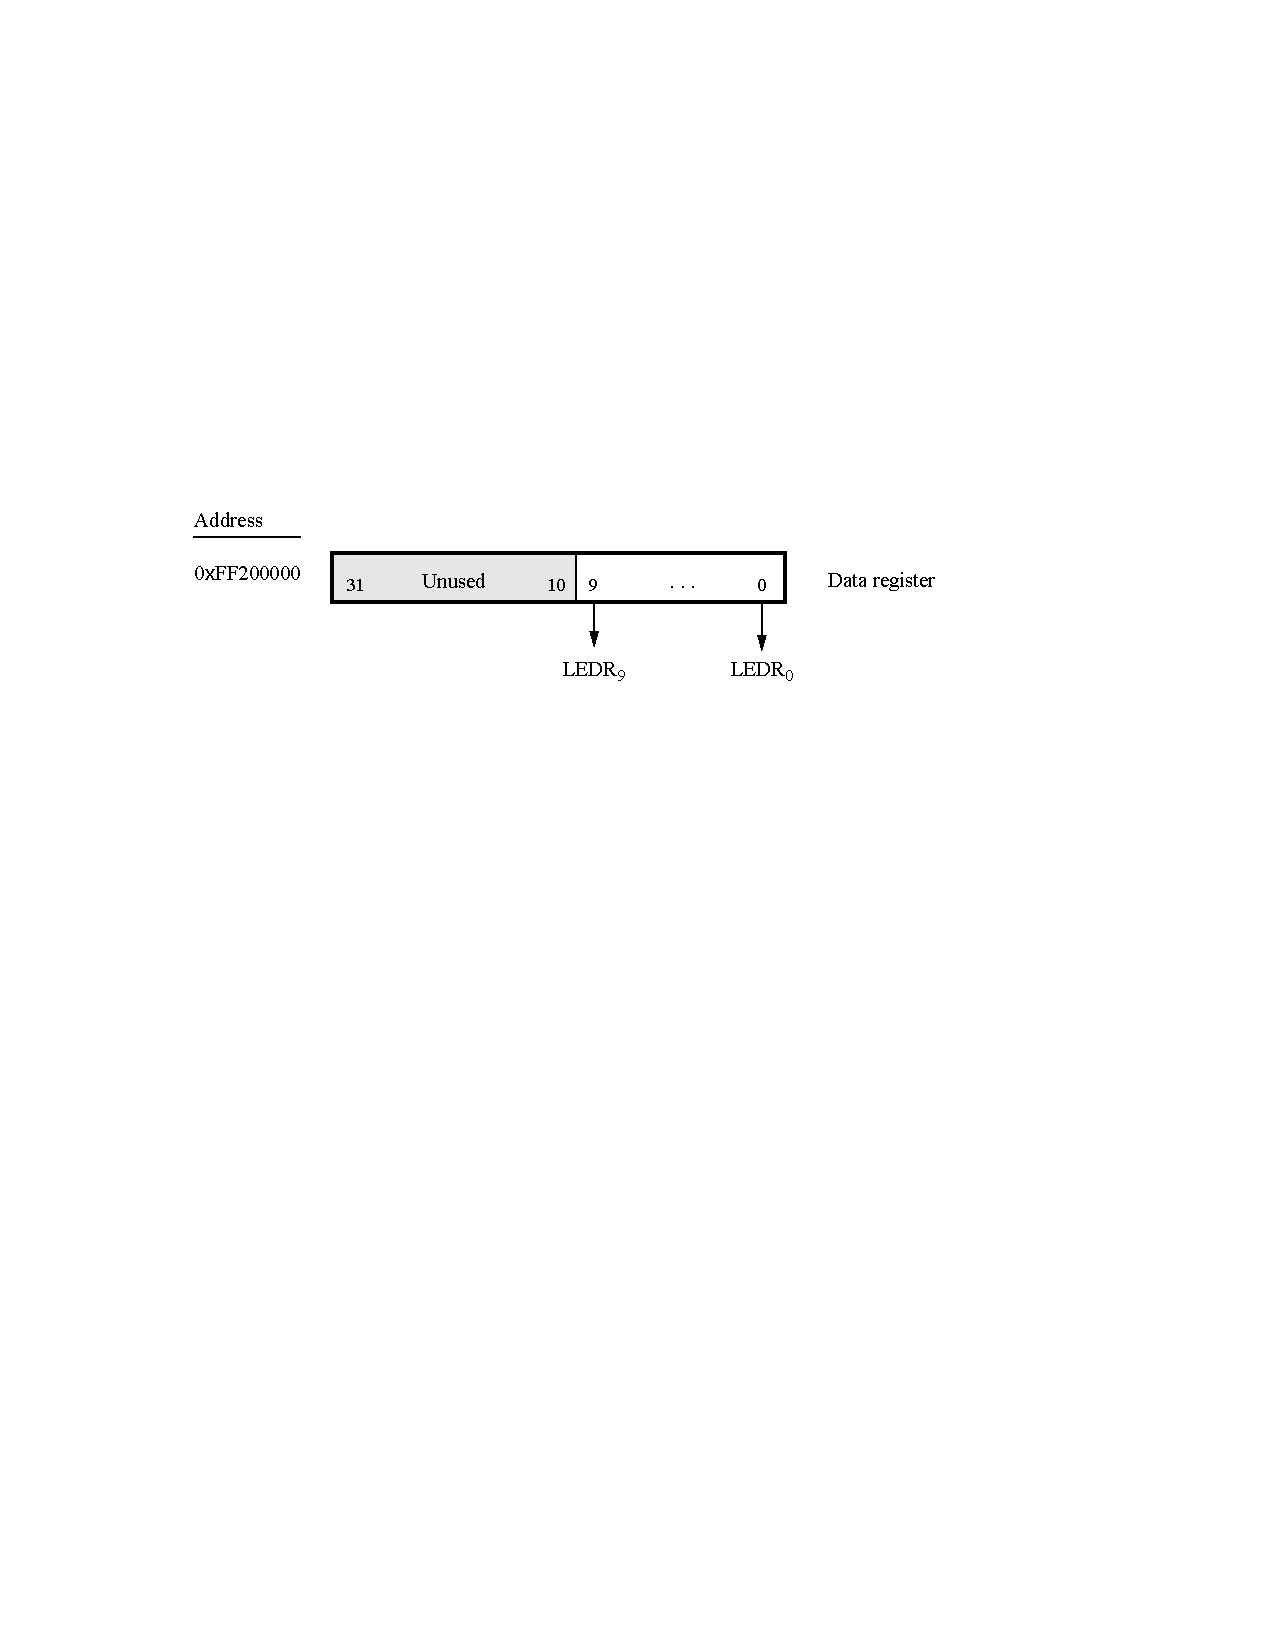
\includegraphics{figures/fig_LED_port.pdf}
   \end{center}
   \caption{The LED parallel port.}
	\label{fig:LED}
\end{figure}

\vspace{-0.25in}
\lstset{language=C,numbers=left}
\begin{figure}[H]
\begin{center}
\begin{minipage}[t]{16 cm}
\begin{lstlisting}
#include <stdio.h>
#include <fcntl.h>
#include <sys/mman.h>
#include "../address_map_arm.h"

/* Prototypes for functions used to access physical memory addresses */
int open_physical (int);
void * map_physical (int, unsigned int, unsigned int);
void close_physical (int);
int unmap_physical (void *, unsigned int);

/* This program increments the contents of the red LED parallel port */
int main(void)
{
   volatile int * LEDR_ptr; // virtual address pointer to red LEDs
   int fd = -1;             // used to open /dev/mem
   void *LW_virtual;        // physical addresses for light-weight bridge
    
   // Create virtual memory access to the FPGA light-weight bridge
   if ((fd = open_physical (fd)) == -1)
      return (-1);
   if (!(LW_virtual = map_physical (fd, LW_BRIDGE_BASE, LW_BRIDGE_SPAN)))
      return (-1);

   // Set virtual address pointer to I/O port
   LEDR_ptr = (int *) (LW_virtual + LEDR_BASE);
   *LEDR_ptr = *LEDR_ptr + 1; // Add 1 to the I/O register
    
   unmap_physical (LW_virtual, LW_BRIDGE_SPAN);
   close_physical (fd);
   return 0;
}
\end{lstlisting}
\end{minipage}
\end{center}
\vspace{-0.33in}\caption{C-code for the {\it increment\_leds} program}
\label{fig:increment_leds_code}
\end{figure}

\begin{itemize} \itemsep1pt \parskip0pt \parsep0pt
\item Lines 2-3 include the \texttt{fcntl.h} and \texttt{sys/mman.h} header files, which are 
needed to use the {\it /dev/mem} device file and the \textit{mmap} and 
\textit{munmap} kernel functions.
\item Line 4 includes the file \texttt{address\_map\_arm.h}, which specifies address offsets 
for all of the FPGA I/O devices that are implemented in the DE1-SoC Computer. The contents of 
this file are listed in Appendix B.
\item Lines 7-10 provide prototype declarations for functions that are used to access physical 
memory. These functions are listed in Figure~\ref{fig:functions}. The functions 
\texttt{open\_physical} and \texttt{close\_physical} are used to open and close the 
{\it /dev/mem} device file. The function {\it map\_physical} calls the \texttt{mmap} kernel 
function to create a physical-to-virtual address mapping for I/O devices, and the 
\texttt{unmap\_physical} closes this mapping. These four functions can be used in any program 
that needs to access physical memory addresses, along with the address information given
in Appendix B.
\newpage
\item Line 20 opens the file \textit{/dev/mem}
\item Line 22 maps a part of the \textit{/dev/mem} file into memory. It maps 
a portion that starts at the base address of {\it lwhps2fpga}, specified in the code as 
\texttt{LW\_BRIDGE\_BASE}, and spans \texttt{LW\_BRIDGE\_SPAN} bytes. Appendix B gives the
values of \texttt{LW\_BRIDGE\_BASE} and \texttt{LW\_BRIDGE\_SPAN}. 
The \texttt{LW\_virtual} variable 
will be set to an address that maps to the bottom of the requested physical address space 
(\texttt{LW\_BRIDGE\_BASE}). 
This means that an access to \texttt{LW\_virtual + offset} will access the physical address 
\texttt{0xFF200000 + offset}.
\item Line 26 calculates the virtual address that maps to the LED port. This is done by adding 
the address offset of the port, \texttt{LEDR\_BASE}, to \texttt{LW\_virtual}.
\item Line 27 reads the \textit{data} register of the LED port, increments the value by 
one, then writes the incremented value back to the register.
\item Lines 29-30 unmap and close the {\it /dev/mem} file
\end{itemize}

\lstset{language=C,numbers=none}
\begin{figure}[H]
\begin{center}
\begin{minipage}[t]{16 cm}
\begin{lstlisting}
/* Open /dev/mem to give access to physical addresses */
int open_physical (int fd) {
   if (fd == -1) // check if already open
      if ((fd = open( "/dev/mem", (O_RDWR | O_SYNC))) == -1) {
         printf ("ERROR: could not open \"/dev/mem\"...\n");
         return (-1);
      }
   return fd;
}

/* Close /dev/mem to give access to physical addresses */
void close_physical (int fd) {
   close (fd);
}

/* Establish a virtual address mapping for the physical addresses starting 
 * at base and extending by span bytes  */
void* map_physical(int fd, unsigned int base, unsigned int span) {
   void *virtual_base;
   // Get a mapping from physical addresses to virtual addresses
   virtual_base = mmap (NULL, span, (PROT_READ | PROT_WRITE), MAP_SHARED, fd, base);
   if (virtual_base == MAP_FAILED) {
      printf ("ERROR: mmap() failed...\n");
      close (fd);
      return (NULL);
   }
   return virtual_base;
}
\end{lstlisting}
\end{minipage}
\end{center}
\vspace{-0.33in}\caption{Functions for managing physical memory addresses (Part $a$).}
\label{fig:functions}
\end{figure}

\lstset{language=C,numbers=none}
\begin{center}
\begin{minipage}[t]{13.5 cm}
\begin{lstlisting}
/* Close the previously-opened virtual address mapping */
int unmap_physical(void * virtual_base, unsigned int span) {
   if (munmap (virtual_base, span) != 0) {
      printf ("ERROR: munmap() failed...\n");
      return (-1);
   }
   return 0;
}
\end{lstlisting}
Figure \ref{fig:functions}. Functions for managing physical memory addresses (Part $b$).
\end{minipage}
\end{center}

\subsection{Device Drivers}
\label{sec:device_drivers}

Device drivers in Linux are software programs that provide an interface to hardware devices. 
There are two types of device drivers: code that is pre-compiled and distributed with
the Linux kernel, and code that is created as a {\it module} that can be added to the kernel at
runtime. We provide an example of a kernel {\it module} in this section; making pre-compiled device 
drivers that are distributed with the Linux kernel is beyond the scope of this tutorial. 

The kernel module described in this section uses the pushbutton KEY port in the DE1-SoC 
Computer. To make the example more interesting, we use ARM processor interrupts to handle
KEY presses. A diagram of the pushbutton KEY port is shown in
Figure~\ref{fig:KEY}. There is a {\it Data} register that reflects which KEY(s) are pressed at
a given time. For example, if {\it KEY}$_0$ is currently being pressed, then bit 0 of the data 
register will be 1, otherwise 0. The {\it Edgecapture} register can be used to check if a 
{\it KEY} has been pressed since last examined, even if it has since been released. If, for 
example, {\it KEY}$_0$ is pressed, then bit 0 of the {\it Edgecapture} register becomes 1. 
This bit remains 1 even if {\it KEY}$_0$ is released. To reset the bit to 0, the ARM processor 
has to explicitly write the value 1 into this bit-position of the {\it Edgecapture} register. The
KEY port can send interrupts to the ARM processor. Interrupts can be enabled for each {\it KEY}
separately, using the {\it Interruptmask} register. An interrupt for a {\it KEY} is enabled 
by setting the corresponding bit in the {\it Interruptmask} register to 1.

\begin{figure}[H]
   \begin{center}
       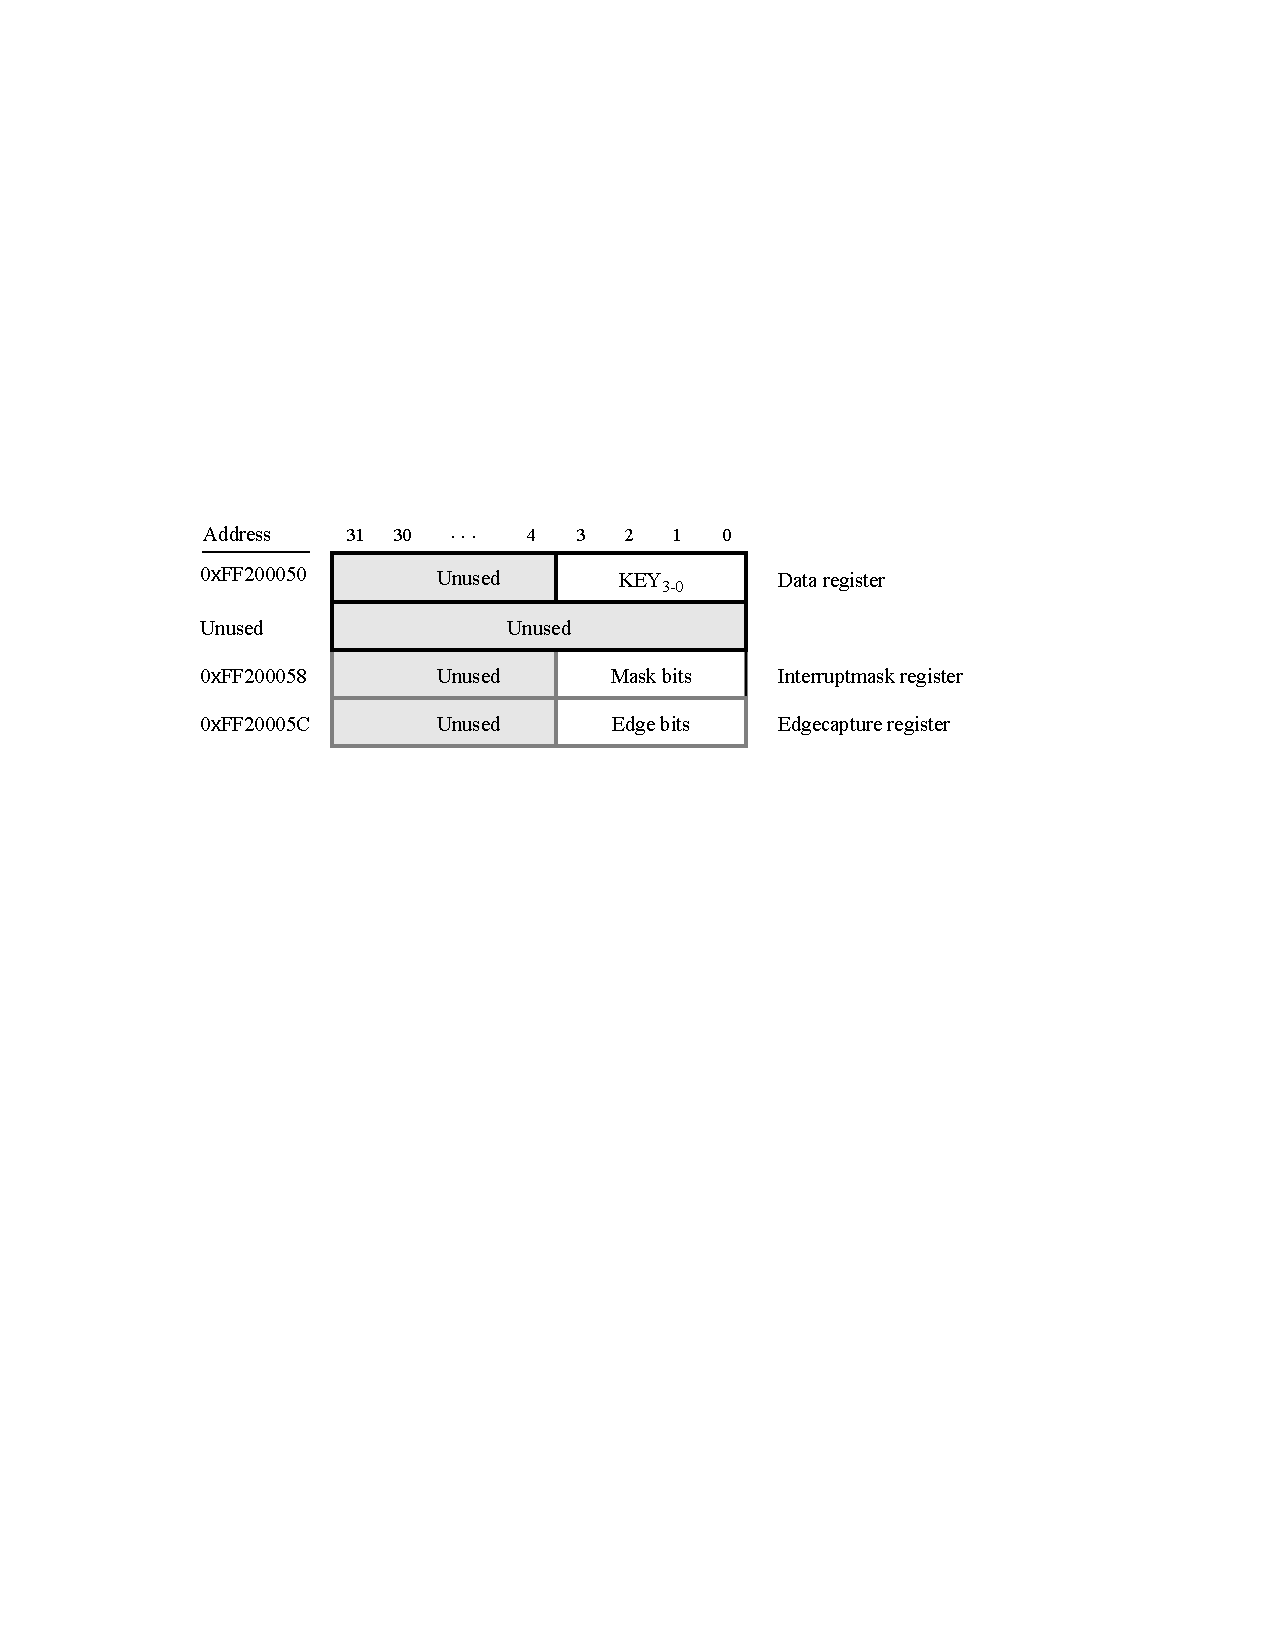
\includegraphics{figures/fig_KEY_port.pdf}
   \end{center}
   \caption{The pushbutton KEY parallel port.}
	\label{fig:KEY}
\end{figure}

Linux allows interrupts to be used only by software code that is part of the kernel. 
The ARM processor of the Cyclone~V device contains a \textit{Generic Interupt Controller} (GIC) 
which can accommodate 256 interrupt request (IRQ) lines IRQ$\,_0$ to IRQ$\,_{255}$. A total of 
64 of the lines (IRQ$\,_{72}$ - IRQ$\,_{135}$) are 
reserved for interrupts originating from hardware devices implemented inside the FPGA. In the 
DE1-SoC Computer the pushbutton KEY port is connected to interrupt line IRQ$\,_{73}$.
This means that our kernel module needs to register an interrupt handler that will respond
to IRQ$\,_{73}$.

Linux contains drivers for the GIC, allowing us to use a high-level interface provided by 
the OS to register an interrupt handler. The Linux header file \texttt{linux/interrupt.h} 
provides this interface, among which is the function \texttt{request\_irq(...)}. This function 
takes an integer argument \texttt{irq} and a function pointer argument \texttt{handler}, and 
registers the function as the handler for IRQ number \texttt{irq}. 

\subsubsection{The Pushbutton Interrupt Handler Kernel Module}

The code for our kernel module is shown in Figure~\ref{fig:pushbutton_irq_handler_code}.
Lines 1-5 in this code include various header files that are needed for our kernel module. 
Line 6 include a file that specifies addresses, and line 7 includes a file that lists all
FPGA interrupts in the DE1-SoC Computer. These files are provided in Appendix B.
Kernel modules, unlike regular C programs, do not have a \texttt{main} function. Instead, 
kernel modules have an \texttt{init} function which is executed when 
the module is inserted into the kernel, and an \texttt{exit} function which is executed if 
the module is removed from the kernel. These functions are specified using the macros 
\texttt{module\_init(...)} and \texttt{module\_exit(...)}. 

The \texttt{init} function in our module is
\texttt{initialize\_pushbutton\_handler(void)}. In this function, line 23 makes a 
{\it system call} to the function \texttt{ioremap\_cache(base\_address, span)}, which is part
of the Linux kernel. This function allows the kernel module to access physical memory
addresses. The \texttt{ioremap\_cache} function has a similar purpose as the 
\texttt{mmap} function that we discussed in Section~\ref{sec:program_with_fpga_communication}.
Kernel modules are not allowed to call the \texttt{mmap} function, and instead have to
use the \texttt{ioremap\_cache} function. This function returns a virtual address that can be 
used to access physical memory starting at {\it base\_address} and extending {\it span} bytes.

Line 25 of the code sets up a virtual address pointer for the LED parallel port, and line
26 initializes the value of this port to \texttt{0x200}, which turns on the leftmost 
LED (as a visual indication that the module has been inserted). The code then configures the 
pushbutton port so that it will generate an interrupt when a button is pressed. Finally, 
line 33 calls \texttt{request\_irq(...)} to register our irq handler \texttt{irq\_handler(...)}
to handle pushbutton interrupts. 
Once registered, \texttt{irq\_handler(...)} is executed whenever the pushbutton port generates 
an interrupt. The handler does two things. First, it increments the value displayed on the 
LEDs to provide visual feedback that the interrupt has been handled. Second, it clears the 
interrupt in the KEY port by writing to the {\it Edgecapture} register.

In this example, \texttt{irq\_handler(...)} serves as a trivial example of an interrupt handler.
A ``real'' driver for a device would do something more useful like transfer data to and from 
buffers, check the status of devices, and the like. A device driver module that does not use
interrupts would still look similar to the code in Figure~\ref{fig:pushbutton_irq_handler_code}, 
but without the interrupt-specific code like \texttt{irq\_handler} and \texttt{free\_irq}.
The \texttt{exit} function in our module is \texttt{cleanup\_pushbutton\_handler(void)}. It sets 
LEDs to \texttt{0x0}, turning them off, and de-registers the pushbutton irq handler by calling 
the \texttt{free\_irq(...)} function. 

\lstset{language=C,numbers=left}
\begin{figure}[H]
\begin{center}
\begin{minipage}[t]{16 cm}
\begin{lstlisting}
#include <linux/kernel.h>
#include <linux/module.h>
#include <linux/init.h>
#include <linux/interrupt.h>
#include <asm/io.h>
#include "../address_map_arm.h"
#include "../interrupt_ID.h"

void * LW_virtual;                 // Lightweight bridge base address
volatile int *LEDR_ptr, *KEY_ptr;  // virtual addresses

irq_handler_t irq_handler(int irq, void *dev_id, struct pt_regs *regs) {
   *LEDR_ptr = *LEDR_ptr + 1;
   // Clear the Edgecapture register (clears current interrupt)
   *(KEY_ptr + 3) = 0xF; 
   return (irq_handler_t) IRQ_HANDLED;
}
static int __init initialize_pushbutton_handler(void) {
   int value;
   // generate a virtual address for the FPGA lightweight bridge
   LW_virtual = ioremap_nocache (LW_BRIDGE_BASE, LW_BRIDGE_SPAN);

   LEDR_ptr = LW_virtual + LEDR_BASE;  // virtual address for LEDR port
   *LEDR_ptr = 0x200;                  // turn on the leftmost light

   KEY_ptr = LW_virtual + KEY_BASE;    // virtual address for KEY port
   *(KEY_ptr + 3) = 0xF; // Clear the Edgecapture register
   *(KEY_ptr + 2) = 0xF; // Enable IRQ generation for the 4 buttons

   // Register the interrupt handler.
   value = request_irq (KEYS_IRQ, (irq_handler_t) irq_handler, IRQF_SHARED, 
      "pushbutton_irq_handler", (void *) (irq_handler));
   return value;
}
static void __exit cleanup_pushbutton_handler(void) {
   *LEDR_ptr = 0; // Turn off LEDs and de-register irq handler
   iounmap (LW_virtual);
   free_irq (KEYS_IRQ, (void*) irq_handler);
}
module_init(initialize_pushbutton_handler);
module_exit(cleanup_pushbutton_handler);
\end{lstlisting}
\end{minipage}
\end{center}
\caption{C-code for the pushbutton interrupt handler kernel module.}
\label{fig:pushbutton_irq_handler_code}
\end{figure}

\subsubsection{Compiling the Kernel Module}

The kernel module source code can be found in the directory
\textit{/home/root/tutorial\_files/pushbutton\_irq\_handler/}. To compile the module, use 
the included Makefile by running the Linux command \texttt{make}. The contents of the Makefile are 
shown in Figure~\ref{fig:pushbutton_irq_handler_makefile}. The first line, 
\texttt{obj-m += <module\_name>.o}, specifies the name of the kernel module that is to be 
built (our kernel module will as a result be named \textit{pushbutton\_irq\_handler}). This 
line also tells the build system to look for the kernel module code in <{\it module\_name}>.c, 
and generate the kernel object file <{\it module\_name}>.{\it ko} at the end of the compilation.
The <{\it module\_name}>.{\it ko} file is a special type of executable program used only
for kernel modules. 

The \texttt{all} target, which is the default target when \texttt{make} is run, calls the 
command \texttt{make -C /lib/modules/\-\$(shell uname -r)/build M=\$(PWD) modules}. 
The \texttt{-C} argument tells the \texttt{make} program to change the working directory 
to \textit{/lib/modules/\$(shell uname -r)/build}, which is the directory containing the source 
code and configuration files of the currently running Linux kernel. In this directory is a 
collection of makefiles called the Linux Kernel Build System (\textit{Kbuild}) that our 
\texttt{make} command leverages to build our kernel module. The remaining arguments 
\texttt{M=\$(PWD)} and \texttt{modules} are used by \textit{Kbuild}.  The argument 
\texttt{M=\$(PWD)} tells \textit{Kbuild} the location of our kernel module source code, 
and \texttt{modules} tells \textit{Kbuild} to build a kernel module. 

The end result of the \texttt{make} command is the generation of 
the \textit{pushbutton\_irq\_handler.ko} kernel module, which is placed in the directory pointed 
to by the \texttt{M=} argument.

\lstset{language=make,numbers=left}
\begin{figure}[H]
\begin{center}
\begin{minipage}[t]{16 cm}
\begin{lstlisting}
obj-m += pushbutton_irq_handler.o
all:
        make -C /lib/modules/$(shell uname -r)/build M=$(PWD) modules
clean:
        make -C /lib/modules/$(shell uname -r)/build M=$(PWD) clean
\end{lstlisting}
\end{minipage}
\end{center}
\caption{Kernel module makefile}
\label{fig:pushbutton_irq_handler_makefile}
\end{figure}

\subsubsection{Using the \texttt{make} Tool}

The \texttt{make} tool provides a convenient mechanism for compiling and building programs,
because \texttt{make} only compiles the parts of a program that have been updated since the 
last time the program was compiled. This mechanism relies on the ability of \texttt{make} 
to check the time- and date-stamp of files and compare them to the current time and date of
the Linux system. On your DE1-SoC board this mechanism can fail to work properly, because the 
board does not have a battery that would allow it to save the current date and time when 
powered off. If the board is reset by pressing the power button, then the Linux system 
will reboot and the date and time will be reverted to to the "Linux epoch", which is 
\texttt{January 1, 1970 00:00:00}. After the date and time have been reverted
the \texttt{make} program will not be able to properly check time 
stamps on files when you compile programs---your files will appear to have dates/times that
are ``in the future''. One way to address this issue is to manually update the date and time
after  Linux has been rebooted, to the current date and time. For example, if the date and time 
is October 15, 2017 at 2:10 pm, you would type the Linux command 
\texttt{date -s "10/15/2017 14:10:00"}. If you consistently set the date and time whenever
Linux is rebooted, the make program should work properly.

\subsubsection{Running the Kernel Module}

A kernel module is executed by {\it inserting} it into the Linux kernel using the command
{\it insmod <module\_name.ko>}. Insert the kernel module you compiled above by
using the command \texttt{insmod pushbutton\_irq\_handler.ko}, as shown in
Figure~\ref{fig:kernel_module_2}. You can use the command {\it lsmod} to confirm that 
your module has been loaded. Once the module is inserted, you should see that the leftmost
red LED on the DE1-SoC board is turned on. Now press any of the four push buttons to generate 
an interrupt on IRQ$\,_{73}$, and confirm that the value displayed on the LEDs increments by one. 

To stop a kernel module, you can remove it from the kernel by using the command
\texttt{rmmod <module\_name>}. Remove your module using the command \texttt{rmmod
pushbutton\_irq\_handler}. You can use the \texttt{lsmod} command to confirm that 
the \textit{pushbutton\_irq\_handler} module has been removed.

\begin{figure}[H]
   \begin{center}
       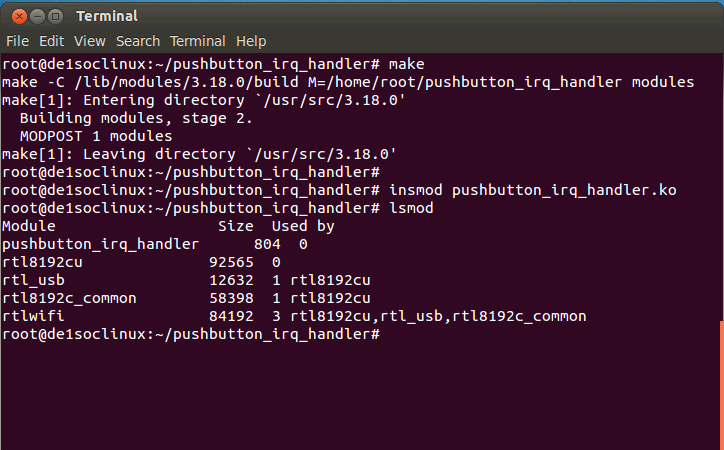
\includegraphics[scale=0.7]{figures/insmod.png}
   \end{center}
   \caption{Inserting and removing the kernel module}
	\label{fig:kernel_module_2}
\end{figure}

\subsubsection{Using Intel\textsuperscript{\textregistered} FPGA Device Drivers}

\noindent In addition to being able to create your own kernel modules, as 
discussed above, the \textit{DE1-SoC-UP} Linux distribution provides a number of pre-built
kernel modules that are available for communicating with hardware modules in the DE1-SoC 
Computer. These pre-built modules are listed in Table 1.

Each of the kernel modules listed in Table 1 provides a {\it character device driver} for
accessing a port in the DE1-SoC Computer. This means that each module has a file-based
interface that can be used to read information from the driver, or write information to
it. The file-based interface is provided in the folder \texttt{/dev/IntelFPGAUP}. One way to
read from a driver is to use the Linux \texttt{cat} command. For example, to read the
states of the pushbutton switches you can type \texttt{cat /dev/IntelFPGAUP/KEY}. Usage 
information for each driver can be found by writing \texttt{-$\,$-} to the driver. For example, 
to see how to use the video driver you could type the Linux command
\texttt{echo -$\,$- > /dev/IntelFPGAUP/video}. 

The drivers listed in Table 1 are not inserted into the Linux kernel during the boot
process. To insert a driver, navigate to the directory
\texttt{/home/root/Linux\_Libraries/drivers}. To insert a specific driver, you can use the
Linux command \texttt{insmod}. For example to insert the \texttt{KEY} driver you would
type \texttt{insmod KEY.ko}. To insert all available drivers, you can execute the script
\texttt{load\_drivers}. Similarly, you can then remove an individual driver by using the
command \texttt{rmmod}, or remove all of the drivers by executing the script
\texttt{remove\_drivers}.

For convenience, a set of {\it wrapper} functions is provided in the C language for use with 
each character device driver. To use these functions in a program, you need 
to provide the statement \texttt{\#include "IntelFPGAUP/{\it xxx}.h"} in your C code, 
where {\it xxx} is the name of the driver from Table 1 (\texttt{KEY}, \texttt{SW}, $\ldots$). 
In addition, you have to append the option \texttt{-lintelfpgaup} to the \texttt{gcc} command when 
compiling your code. The contents of the files {\it xxx.h}, which list all of the 
available wrapper functions, are shown in Appendix C. An example of a C program that uses 
these wrapper functions is given in Appendix D. If this program is stored in a file 
name {\it draw\_lines.c}, then you would compile it with a command such as 
\texttt{gcc -Wall -o draw\_lines draw\_lines.c -lintelfpgaup}. The wrapper source code
files and examples can be found in the directory \texttt{$\sim$/Linux\_Libraries/C4DE}.

A set of wrapper functions is also provided in the Python* language for use with each character 
device driver. To use these functions in a Python program you need to include the 
statement \texttt{import} {\it xxx}, where {\it xxx} is the name of the device from Table 1. 
You also need to have the proper setting in your \texttt{PYTHONPATH} environment variable so that
the Python interpreter can locate the wrapper functions. The contents of the Python 
wrappers {\it xxx.py}, which list all of the available wrapper functions, are shown in 
Appendix E. An example of a program that uses these wrapper functions is given in Appendix F.
The wrapper source code files and example programs are included in the directory
$\sim$/Linux\_Libraries/PyDE.

To check your \texttt{PYTHONPATH} variable you can execute the 
Linux command \texttt{echo \$PYTHONPATH}.
If the path variable does not include the directory \texttt{$\sim$/Linux\_Libraries/PyDE/src},
then in the file \texttt{$\sim$/.bash\_profile} add the line 
\texttt{export PYTHONPATH=:/home/root/Linux\_Libraries/PyDE/src}. This statement assumes 
that your home directory is \texttt{/home/root}. If not, then substitute the appropriate 
directory name. Finally, include the new setting in your current login session by executing 
the command \texttt{source $\sim$/.bash\_profile}. 

\begin{table}
\centering
\begin{tabular}{l|p{8cm}}
{\bf Kernel module}	&	{\bf Description}\\\hline
\rule{0cm}{.5cm}\texttt{KEY}	&	Used to access the pushbutton KEY port\\
\texttt{SW}		&	Used to access the slide switch SW port\\
\texttt{LEDR}	&	Used to access the red light LEDR port\\
\texttt{HEX}	&	Used to access the seven-segment HEX display port\\
\texttt{video}	&	Used to access the VGA video-out port\\
\texttt{audio}	&	Used to access the digital audio port\\
\texttt{accel}	&	Used to access the 3-D accelerometer port\\
\end{tabular}
\center{Table 1. Pre-built kernel modules}
\label{tab:drivers}
\end{table}

\subsubsection*{Drivers for the DE10-Standard Board}

If you are using the DE10-Standard board, then all of the device drivers listed in Table 1
are available, as well as their corresponding wrappers. In addition, there is a device
driver called \texttt{LCD}, which controls the $128 \times 64$ LCD display on the
DE10-Standard board. The wrappers provided for the \texttt{LCD} driver are identical to
those of the video driver in Table 1.

\subsubsection*{Drivers for the DE10-Nano Board}

If you are using the DE10-Nano board, then all of the device drivers listed in Table 1 are
available, except for the \texttt{HEX} driver. Also, for this board the \texttt{LEDR}
driver, and corresponding wrappers, is named \texttt{LED}.

\newpage
\section*{Appendix A~~~~ Using \texttt{Code::Blocks}}

If you have a network connection to your DE1-SoC board, as described in
Section~\ref{sec:conn_network}, then you can make use of the \texttt{Code::Blocks} tool for
developing and debugging application programs. In this appendix we provide a simple example 
that shows how to create a \texttt{Code::Blocks} {\it project}.
We will show how to build a project using the {\it increment\_leds} example that we discussed in
Section~\ref{sec:program_with_fpga_communication}.

Open the \texttt{Code::Blocks} tool by clicking on its icon, which looks like four colored
cubes. The main window of \texttt{Code::Blocks} is displayed in Figure~\ref{fig:cb1}. In this
window, click on \texttt{Create a new project} to begin using the tool. In the window that
opens click on the \texttt{Empty project} item, and then click on the \texttt{Go} button.

In the {\it Empty project} dialog, shown in Figure~\ref{fig:cb3}, type a title for the
project, such as \texttt{increment\_leds}. Use the \texttt{...} button to navigate to, and
select, the folder that contains the {\it increment\_leds} source code. Give the project a
name like {\it increment\_leds}. Make sure that the \texttt{Resulting filename} item shows 
the proper name and path to the project. Click on the \texttt{Next} button to reach a
second \texttt{Empty project} dialog. Then, click \texttt{Finish} to return to the main
\texttt{Code::Blocks} window.

\begin{figure} [h]
\begin{center}
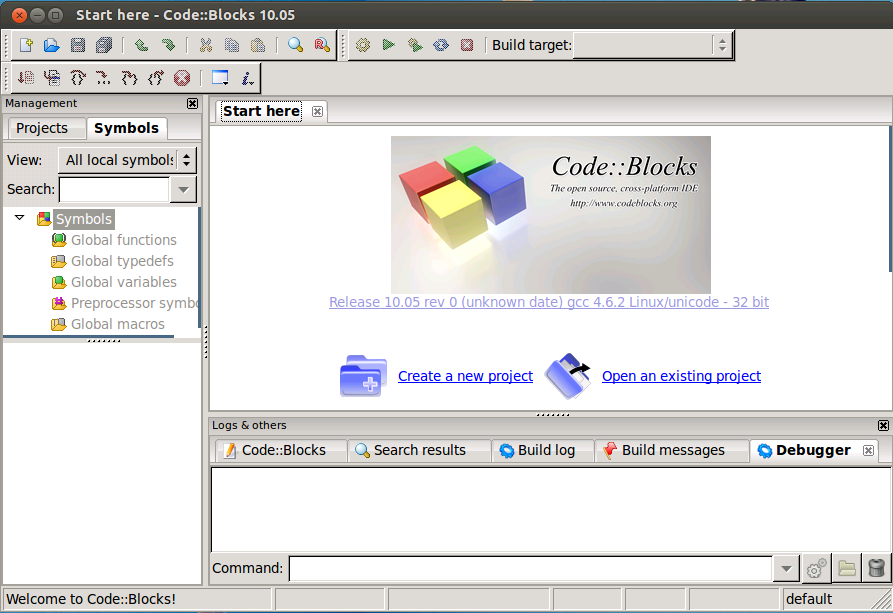
\includegraphics[scale = .60]{figures/cb1.png}
\end{center}
\caption{The main \texttt{Code::Blocks} window.}
\label{fig:cb1}
\end{figure}

\begin{figure} [h]
\begin{center}
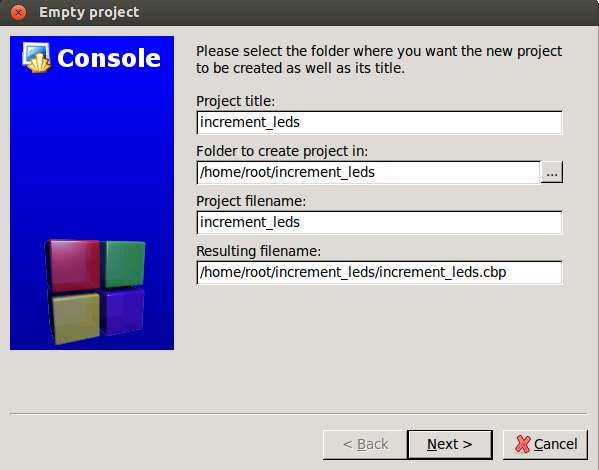
\includegraphics[scale = .60]{figures/cb3.png}
\end{center}
\caption{The \texttt{Empty project} dialog.}
\label{fig:cb3}
\end{figure}

As indicated in Figure~\ref{fig:cb5} right-click the {\it increment\_leds} name under
\texttt{Workspace}, and then select \texttt{Add files...}. Select the {\it
increment\_leds.c} source-code file, as illustrated in Figure~\ref{fig:cb6}, and then 
click the \texttt{Open} button. In the dialog that opens, illustrated in
Figure~\ref{fig:cb7}, select \texttt{OK}. Now you can open the \texttt{increment\_leds} item
under \texttt{Workspace}, then open the \texttt{Sources} sub-menu, and double-click to open 
the {\it increment\_leds.c} file inside the \texttt{Code::Blocks} window. You can change
the size of the displayed text by holding down the \texttt{CTRL} key and scrolling with
the mouse.

\begin{figure} [h]
\begin{center}
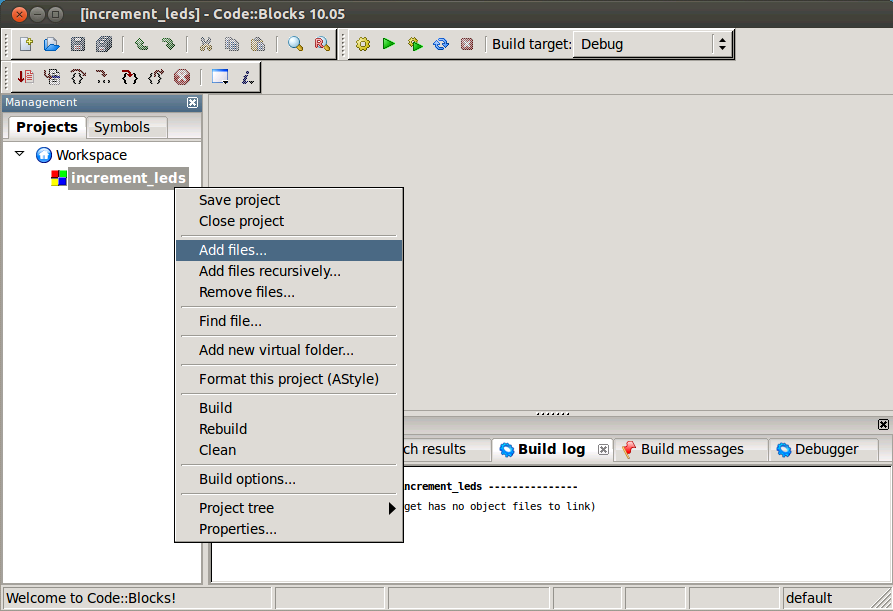
\includegraphics[scale = .60]{figures/cb5.png}
\end{center}
\caption{Adding source-code files to the project.}
\label{fig:cb5}
\end{figure}

\clearpage
\newpage
Click to the right of the line of code that calls the function
\texttt{open\_physical}, as shown in Figure~\ref{fig:cb13},
and set a {\it breakpoint}. The breakpoint is indicated by a red circle. 

Now start the debugger by selecting the command \texttt{Debug $\mid$ Start}, as indicated in 
in Figure~\ref{fig:cb8}. (Note that the main menu commands for \texttt{Code::Blocks} are
provided at the top of the Linux desktop, and not in the border of the
\texttt{Code::Blocks} window.) The debugger will start running the program and it will
stop when the code reaches the breakpoint. Figure~\ref{fig:cb11} shows the debugger window
after reaching the breakpoint. If the \texttt{CPU Registers} window is not visible, it can
be opened by selecting the command \texttt{Debug $\mid$ Debugging windows $\mid$ CPU
Registers}. This window shows the current contents of the ARM processor general-purpose registers.

The debugger can display the values of variables used in your program, as
illustrated in Figure~\ref{fig:cb12}. Expand the \texttt{Local variables} item in the
\texttt{Watches} window to see the variables that currently exist in the program.
Execute a few more lines of code until the value of the {\it LEDR\_ptr} variable is initialized
by the program, as displayed in the figure. To execute a line of code use the command
\texttt{Debug $\mid$ Next line}. This command is available in the main {\it Debug}
menu, via the short-cut keyboard key \texttt{F7}, or by clicking on its icon in the
{\it Debug toolbar}. If this toolbar is not open when the debugger is running, it can be
opened by using the command \texttt{View $\mid$ Toolbars $\mid$ Debugger}.

More complete information about using \texttt{Code::Blocks} can be found by searching
for documentation and tutorials on the Internet.
~\\
\begin{figure} [h]
\begin{center}
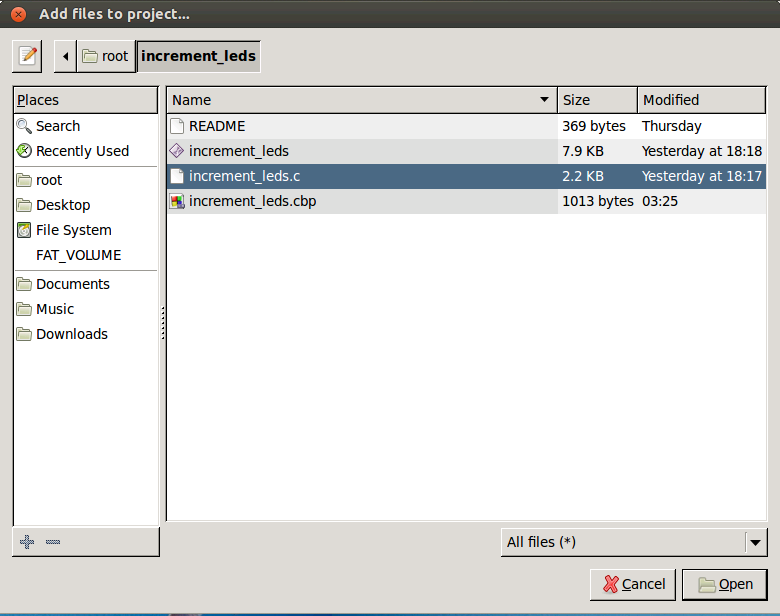
\includegraphics[scale = .60]{figures/cb6.png}
\end{center}
\caption{Selecting the {\it increment\_leds.c} file.}
\label{fig:cb6}
\end{figure}

\begin{figure} [h]
\begin{center}
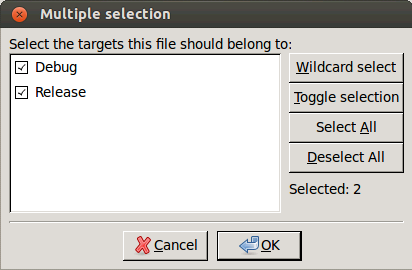
\includegraphics[scale = .60]{figures/cb7.png}
\end{center}
\caption{Selecting build targets.}
\label{fig:cb7}
\end{figure}

\begin{figure} [h]
\begin{center}
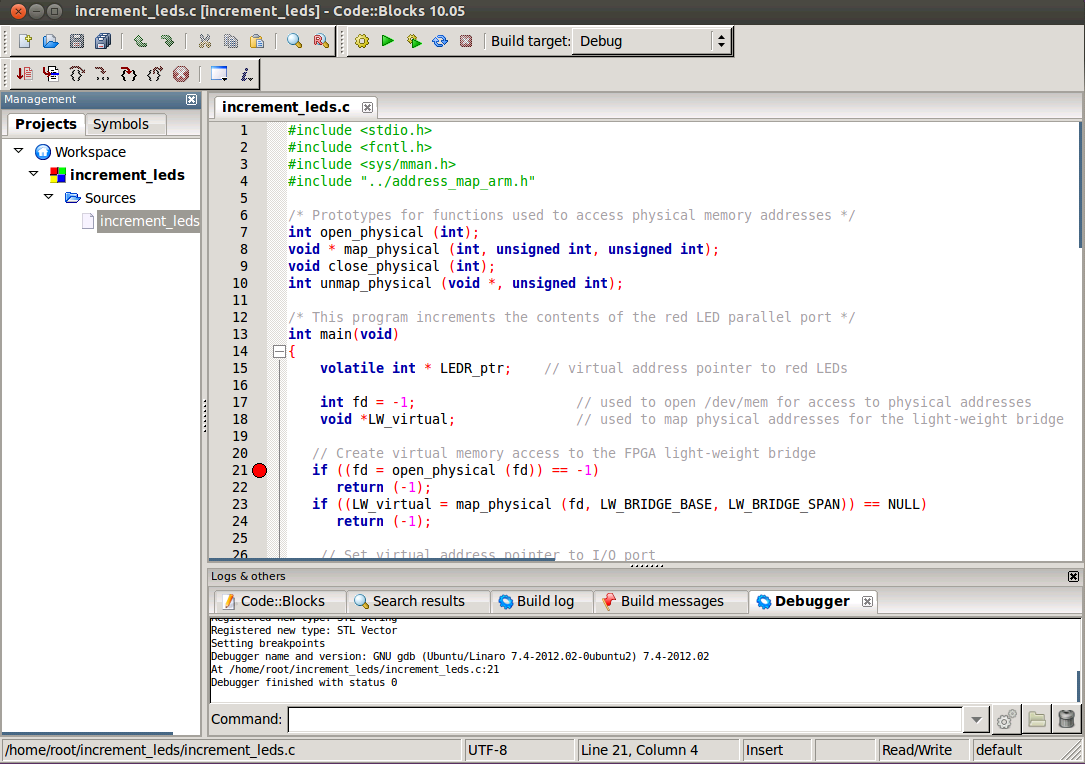
\includegraphics[scale = .55]{figures/cb13.png}
\end{center}
\caption{Setting a breakpoint.}
\label{fig:cb13}
\end{figure}

\begin{figure} [h]
\begin{center}
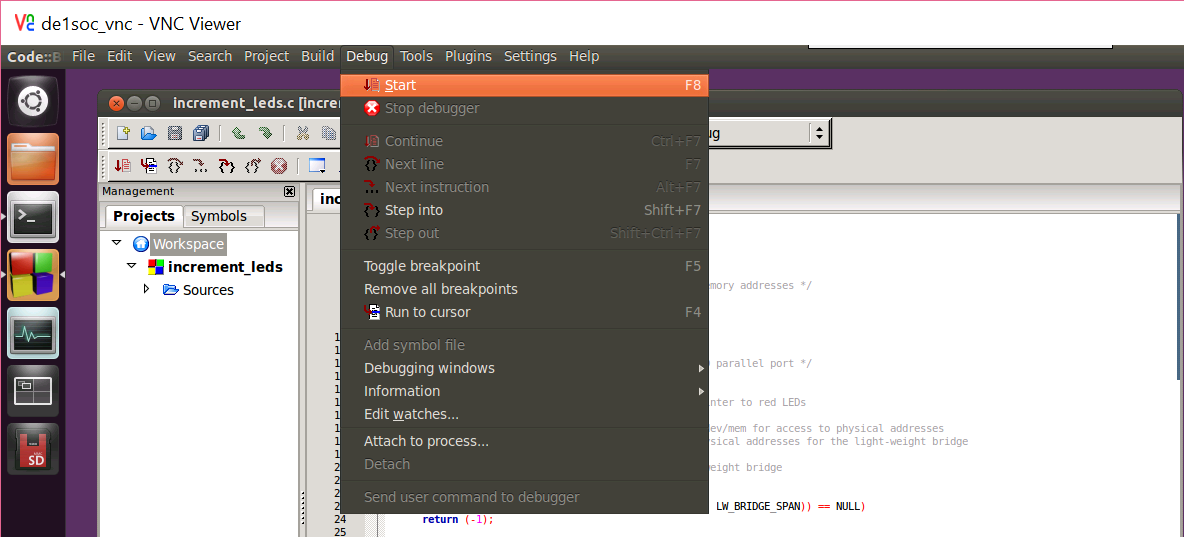
\includegraphics[scale = .55]{figures/cb8.png}
\end{center}
\vspace{-0.5cm}\caption{Starting the debugger.}
\label{fig:cb8}
\end{figure}

\begin{figure} [h]
\begin{center}
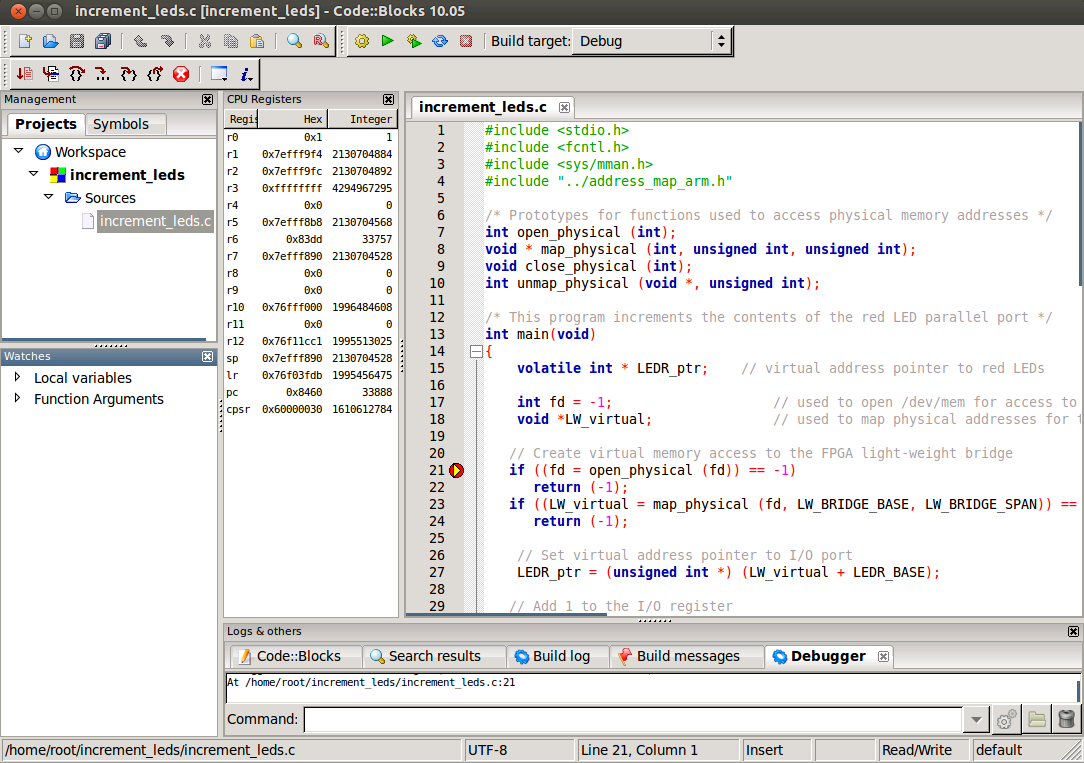
\includegraphics[scale = .55]{figures/cb11.png}
\end{center}
\caption{The debugging window.}
\label{fig:cb11}
\end{figure}

\clearpage
\newpage
\begin{figure} [h]
\begin{center}
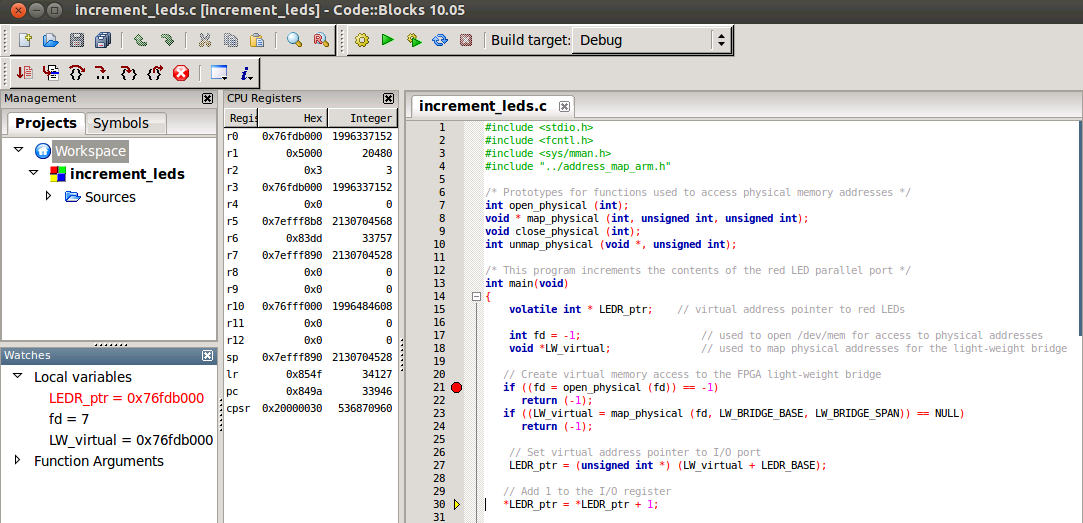
\includegraphics[scale = .55]{figures/cb12.png}
\end{center}
\caption{Displaying the values of variables.}
\label{fig:cb12}
\end{figure}

\newpage
\section*{Appendix B~~~~Include Files}

Figure~\ref{fig:address_map} shows the contents of the {\it include} file {\it address\_map\_arm.h}
that is discussed in Section~\ref{sec:program_with_fpga_communication}. This file lists
memory and FPGA I/O addresses in the DE1-SoC Computer. 

\lstset{language=C,numbers=none}
\begin{figure}[H]
\begin{center}
\begin{minipage}[t]{16 cm}
\begin{lstlisting}
/* Memory */
#define DDR_BASE              0x00000000
#define DDR_SPAN              0x3FFFFFFF
#define A9_ONCHIP_BASE        0xFFFF0000
#define A9_ONCHIP_SPAN        0x0000FFFF
#define SDRAM_BASE            0xC0000000
#define SDRAM_SPAN            0x03FFFFFF
#define FPGA_ONCHIP_BASE      0xC8000000
#define FPGA_ONCHIP_SPAN      0x0003FFFF
#define FPGA_CHAR_BASE        0xC9000000
#define FPGA_CHAR_SPAN        0x00001FFF

/* Cyclone V FPGA devices */
#define LW_BRIDGE_BASE        0xFF200000

#define LEDR_BASE             0x00000000
#define HEX3_HEX0_BASE        0x00000020
#define HEX5_HEX4_BASE        0x00000030
#define SW_BASE               0x00000040
#define KEY_BASE              0x00000050
#define JP1_BASE              0x00000060
#define JP2_BASE              0x00000070
#define PS2_BASE              0x00000100
#define PS2_DUAL_BASE         0x00000108
#define JTAG_UART_BASE        0x00001000
#define JTAG_UART_2_BASE      0x00001008
#define IrDA_BASE             0x00001020
#define TIMER0_BASE           0x00002000
#define TIMER1_BASE           0x00002020
#define AV_CONFIG_BASE        0x00003000
#define PIXEL_BUF_CTRL_BASE   0x00003020
#define CHAR_BUF_CTRL_BASE    0x00003030
#define AUDIO_BASE            0x00003040
#define VIDEO_IN_BASE         0x00003060
#define ADC_BASE              0x00004000

#define LW_BRIDGE_SPAN        0x00005000
\end{lstlisting}
\end{minipage}
\end{center}
\caption{The contents of the file {\it address\_map\_arm.h}.}
\label{fig:address_map}
\end{figure}

\newpage
Figure~\ref{fig:interrupts} shows the contents of the {\it include} file {\it interrupt\_ID.h}
that is discussed in Section~\ref{sec:device_drivers}. This file lists
the FPGA interrupt line numbers in the DE1-SoC Computer. 

\lstset{language=C,numbers=none}
\begin{figure}[H]
\begin{center}
\begin{minipage}[t]{16 cm}
\begin{lstlisting}
/* FPGA interrupts */
#define   TIMER0_IRQ             72
#define   KEYS_IRQ               73
#define   TIMER1_IRQ             74
#define   FPGA_IRQ3              75
#define   FPGA_IRQ4              76
#define   FPGA_IRQ5              77
#define   AUDIO_IRQ              78
#define   PS2_IRQ                79
#define   JTAG_IRQ               80
#define   IrDA_IRQ               81
#define   FPGA_IRQ10             82
#define   JP1_IRQ                83
#define   JP2_IRQ                84
#define   FPGA_IRQ13             85
#define   FPGA_IRQ14             86
#define   FPGA_IRQ15             87
#define   FPGA_IRQ16             88
#define   PS2_DUAL_IRQ           89
#define   FPGA_IRQ18             90
#define   FPGA_IRQ19             91
\end{lstlisting}
\end{minipage}
\end{center}
\caption{The contents of the file {\it interrupt\_ID.h}.}
\label{fig:interrupts}
\end{figure}

\newpage
\section*{Appendix C~~~~ Wrapper Functions for using Character Device Drivers with C Code}

\subsection*{Header File for Pushbutton KEY Device}
\lstset{language=C,numbers=none}
\lstinputlisting{C4DE/include/KEY.h}
\newpage
\subsection*{Header File for Slide Switch SW Device}
\lstinputlisting{C4DE/include/SW.h}
\newpage
\subsection*{Header File for Red Light LEDR Device}
\lstinputlisting{C4DE/include/LEDR.h}
\newpage
\subsection*{Header File for Seven-Segment HEX Device}
\lstinputlisting{C4DE/include/HEX.h}
\newpage
\subsection*{Header File for VGA Video Device}
\lstinputlisting{C4DE/include/video.h}
\newpage
\subsection*{Header File for Digital Audio Device}
\lstinputlisting{C4DE/include/audio.h}
\newpage
\subsection*{Header File for 3-D Accelerometer Device}
\lstinputlisting{C4DE/include/accel.h}

\newpage
\section*{Appendix D~~~~ Example C Program Using Device Drivers}

\lstinputlisting{C4DE/examples/draw_lines/draw_lines.c}

\newpage
\section*{Appendix E~~~~ Wrapper Functions for using Character Device Drivers with Python* Code}

\subsection*{Pushbutton KEY Device: KEY.py}
\lstset{language=Python,numbers=none}
\lstinputlisting{PyDE/include/KEY.py}
\newpage
\subsection*{Slide Switch SW Device: SW.py}
\lstinputlisting{PyDE/include/SW.py}
\newpage
\subsection*{Red Light LEDR Device: LEDR.py}
\lstinputlisting{PyDE/include/LEDR.py}
\newpage
\subsection*{Seven-Segment HEX Device: HEX.py}
\lstinputlisting{PyDE/include/HEX.py}
\newpage
\subsection*{VGA Video Device: video.py}
\lstinputlisting{PyDE/include/video.py}
\newpage
\subsection*{Digital Audio Device: audio.py}
\lstinputlisting{PyDE/include/audio.py}
\newpage
\subsection*{3-D Accelerometer Device: accel.py}
\lstinputlisting{PyDE/include/accel.py}

\newpage
\section*{Appendix F~~~~ Example Python* Program Using Device Drivers}

\lstinputlisting{PyDE/examples/draw_lines/draw_lines.py}

\newpage
\section*{Appendix G~~~~FPGA Configuration}

A special mechanism built into the Cyclone V SoC allows software running on the ARM processor
(such as the Linux OS) to program the FPGA. The \textit{DE1-SoC-UP} Linux distribution contains 
drivers for this mechanism, allowing us to program the FPGA from the Terminal window. The 
following sections describe how to use this mechanism.

\subsubsection*{Creating an RBF Programming File}
\label{sec:create_rbf_file}

The FPGA programming mechanism accepts an input FPGA bitstream in the \textit{Raw Binary File} (.rbf) file format. This means that once you compile your circuit using Quartus\textsuperscript{\textregistered}, which outputs the FPGA bitstream in the \textit{SRAM Object File} (.sof) file format, you must convert the .sof file into a .rbf file. This is done using Quartus's \textit{Convert Programming File} tool, and the steps are described below.

\begin{enumerate}
\item Launch the Convert Programming File tool by selecting \texttt{File $>$ Convert Programming Files...}.
\item Select \texttt{Raw Binary File (.rbf)} as the \texttt{Programming file type}.
\item Select \texttt{Passive Parallel x16} as the \texttt{Mode}.
\item Specify the destination file name in the \texttt{File name} field.
\item Click and highlight \texttt{SOF Data} then add the .sof file that you wish to
convert by clicking \texttt{Add File...}.

\begin{figure}[h]
   \begin{center}
       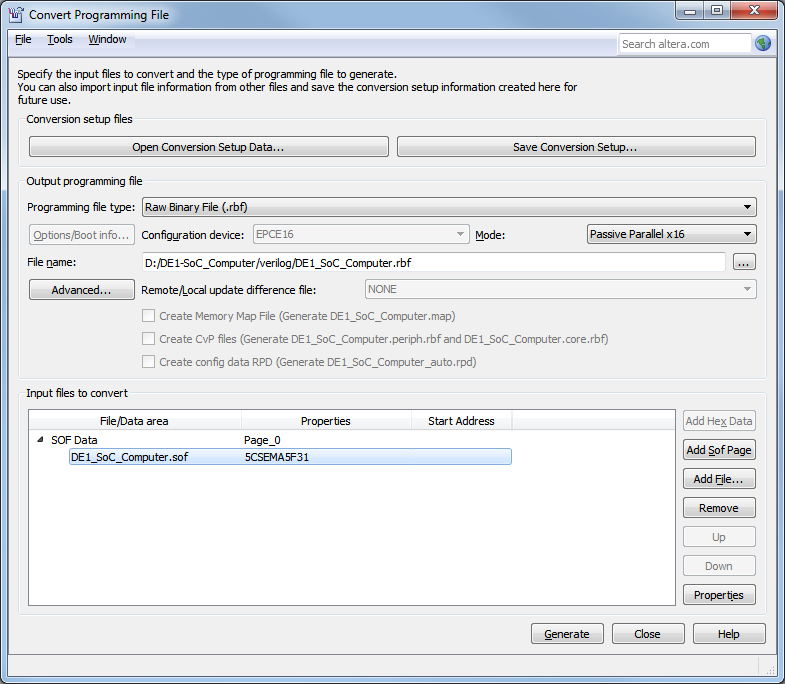
\includegraphics[scale=0.7]{figures/rbf_conversion_1}
   \end{center}
   \caption{The Convert Programming File Tool.}
	\label{fig:rbf_conversion_1}
\end{figure}

\item Click and highlight the newly added .sof file in the list, then select
\texttt{Properties}. You should see the window shown in Figure~\ref{fig:rbf_conversion_2}. 
Enable file compression by ticking the checkbox as shown, then press OK.
\item We are now ready to generate the .{\it rbf} file. Click \texttt{Generate}. You should
see the success message shown in Figure~\ref{fig:rbf_conversion_3}. 
\item Finally, we can transfer the .{\it rbf} file to the Linux file system, using a method such 
as ftp.
\end{enumerate}

\subsubsection*{Programming the FPGA}
\label{sec:program_fpga}

While Linux boots, scripts are executed to initialize various Linux components. One of these 
scripts, located at {\it /etc/init.d/programfpga}, programs the FPGA with the default 
programming file {\it /home/root/DE1\_SoC\_Computer.rbf}. If you examine the contents of
the {\it programfpga} script, you will see that it comprises the commands 

\lstset{language=sh,numbers=none,escapechar=\%}
\begin{center}
\begin{minipage}[t]{16 cm}
\begin{lstlisting}
echo 0 > /sys/class/fpga-bridge/fpga2hps/enable
echo 0 > /sys/class/fpga-bridge/hps2fpga/enable
echo 0 > /sys/class/fpga-bridge/lwhps2fpga/enable
dd %if%=/home/root/DE1_SoC_Computer.rbf of=/dev/fpga0 bs=1M
echo 1 > /sys/class/fpga-bridge/fpga2hps/enable
echo 1 > /sys/class/fpga-bridge/hps2fpga/enable
echo 1 > /sys/class/fpga-bridge/lwhps2fpga/enable
\end{lstlisting}
\end{minipage}
\end{center}

The .{\it rbf} file is loaded into the FPGA device using the command
\lstset{language=sh,numbers=none,escapechar=\%}
\begin{lstlisting}
dd %if%=<filename> of=/dev/fpga0 bs=1M
\end{lstlisting}
where the input \texttt{<filename>} is \texttt{ /home/root/DE1\_SoC\_Computer.rbf}. To program 
a different file into the FPGA you need to execute the above commands, and specify 
whatever .{\it rbf} file is wanted. 

\begin{figure}[H]
   \begin{center}
       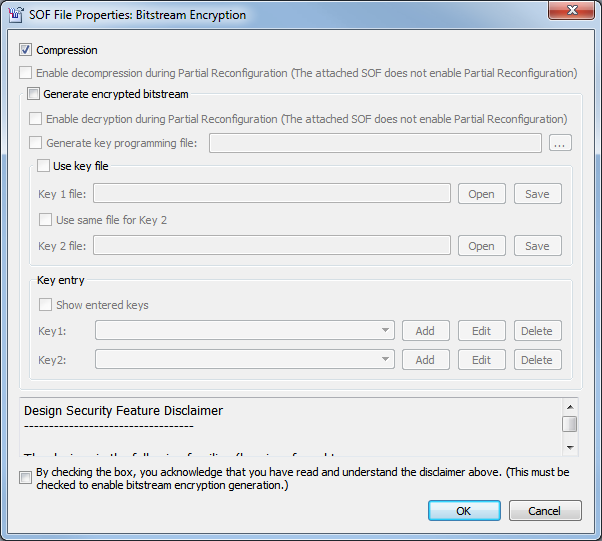
\includegraphics[scale=0.7]{figures/rbf_conversion_2}
   \end{center}
   \caption{Enabling file compression.}
	\label{fig:rbf_conversion_2}
\end{figure}
\begin{figure}[H]
   \begin{center}
       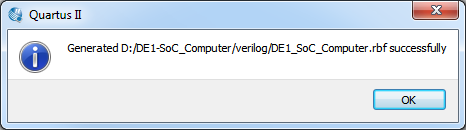
\includegraphics[scale=0.7]{figures/rbf_conversion_3}
   \end{center}
   \caption{The .rbf file successfully generated.}
	\label{fig:rbf_conversion_3}
\end{figure}

% Copyright and Trademark

%\newcommand{\datePublished}{Mar 2022}

\newcommand{\versnum}{21.1} %version number quartus/AMP
\newcommand{\quartusname}{Quartus\textsuperscript{\textregistered} Prime}	
\newcommand{\textBar}{For \quartusname{} \versnum{}}
\newcommand{\thisyear}{2022 } %for copyright
\newcommand{\company}{FPGAcademy.org}
\newcommand{\longteamname}{FPGAcademy.org}
\newcommand{\teamname}{FPGAcademy}
\newcommand{\website}{FPGAcademy.org}

\newcommand{\productAcronym}{AMP}
\newcommand{\productNameShort}{Monitor Program}

\newcommand{\productNameMedTM}{Monitor Program}
\newcommand{\productNameMed}{Monitor Program}

%\newcommand{\headerLogoFilePath}[1]{#1/FPGAcademy.png}



%%%%%%%%%%%%%%%%%%%%%%%%%%%%%%%%%%%%%%%%
%%% FPGAcademy Copyright Information %%%
%%%%%%%%%%%%%%%%%%%%%%%%%%%%%%%%%%%%%%%%

%Always put the copyright on a new page (clear page), with some vertical space from top
\clearpage
\vspace{1in}

\noindent

Copyright {\copyright} FPGAcademy.org. All rights reserved. FPGAcademy and the FPGAcademy logo are trademarks of  FPGAcademy.org.  This document is being provided on an ``as-is'' basis and as an accommodation and therefore all warranties, representations or guarantees of any kind (whether express, implied or statutory) including, without limitation, warranties of merchantability, non-infringement, or fitness for a particular purpose, are specifically disclaimed.

%FPGAcademy assumes no responsibility or liability arising out of the application or use of any information,  product,  or  service  described  herein  except  as  expressly  agreed  to  in  writing  by  FPGAcademy.



**Other names and brands may be claimed as the property of others.





\end{document}

